\documentclass[12pt]{{memoir}}
\usepackage{graphicx}
\usepackage[overlay]{textpos}
\usepackage[hidelinks,pdfusetitle]{hyperref}
\usepackage{amsmath}
\usepackage{longtable}
\usepackage{pbox}
\usepackage{xfrac}
\usepackage[paperwidth=7.5in,paperheight=10.0in,top=.5in,bottom=.5in,left=.25in,right=.25in]{geometry}
\newcommand\scsg[1]{\raisebox{-1.25pt}[8.75pt][1.25pt]{\includegraphics[height=10pt]{char#1}}}

\newcommand\keycaps[1]{\raisebox{0in}[.2734375in][.1015625in]{\tiny\textsf{#1}}}

\newcommand\keycapt[1]{\raisebox{0in}[.28125in][.09375in]{\texttt{#1}}}

\newcommand\Hline{%
\hline\raisebox{0pt}[1.125em]{}}

\newcommand\opdoc[5]{%
\filbreak\subsubsection{\texttt{\large#1} \textmd{\textit{#2}}}
\par#3\par
\begin{center}
#4#5
\end{center}}

\newcommand\flageffects[8]{%
\begin{tabular}[t]{cccccc}
\ifx&#1&%
  \empty
\else
  \multicolumn{6}{c}{\hspace*{-1em}#1\hspace*{-1em}} \\
  \Hline
\fi
\,N\, & \,V\, & \,D\, & \,I\, & \,Z\, & \,C\, \\
#2 & #3 & #4 & #5 & #6 & #7 \\
\ifx&#8&%
  \empty
\else%
  \multicolumn{6}{c}{#8} \\
\fi
\end{tabular}\hspace{1em}}

\newcommand\opeffects[8]{%
\ifx&#2&%
  \ifx&#3&%
    \ifx&#4&%
      \ifx&#5&%
        \ifx&#6&%
          \ifx&#7&%
            {#1}\hspace{1em}
          \else
            \flageffects{#1}{#2}{#3}{#4}{#5}{#6}{#7}{#8}
          \fi
        \else
          \flageffects{#1}{#2}{#3}{#4}{#5}{#6}{#7}{#8}
        \fi
      \else
        \flageffects{#1}{#2}{#3}{#4}{#5}{#6}{#7}{#8}
      \fi
    \else
      \flageffects{#1}{#2}{#3}{#4}{#5}{#6}{#7}{#8}
    \fi
  \else
    \flageffects{#1}{#2}{#3}{#4}{#5}{#6}{#7}{#8}
  \fi
\else
  \flageffects{#1}{#2}{#3}{#4}{#5}{#6}{#7}{#8}
\fi
}

\newcommand\opctable[1]{%
\begin{tabular}[t]{l>{\ttfamily}l>{\ttfamily}ccc}
Addressing & \textrm{Asm syntax} & \textrm{Opcode} & Bytes & Cycles \\
#1
\end{tabular}}

\newcommand\fwsubroutinehdr[1]{%
\filbreak
\subsubsection{#1}}

\newcommand\opcrow[5]{%
#1 & #2 & #3 & #4 & #5\\}

\interfootnotelinepenalty=10000
\begin{document}
\title{Retro 6k Programmer's Guide}
\author{Maggie\,David P.\,K. Haynes}
\pagestyle{empty}
\begin{center}
\includegraphics{logolineart}

\vspace{\stretch{.25}}
{\sffamily\bfseries\Huge{}Retro 6k\\Fantasy Computer\\Entertainment System

\vspace{\stretch{1}}
Programmer's Guide\par}
\vspace*{\stretch{1}}
{\sffamily\bfseries\large\theauthor\par}
\end{center}
\vspace*{\stretch{3}}
\cleartoverso
\vspace*{\stretch{2}}
\begin{center}
\noindent{}Hey, Dad. Thanks for getting \\
me started in computer programming and \\
teaching me about electronics. Could you maybe stop \\
voting for politicians who want to make life \\
harder for people like me?\par
\end{center}

\vspace*{\stretch{3}}
\cleartorecto
\tableofcontents*
\clearpage
\pagestyle{headings}

\vspace*{3in}
\section*{Conventions Used In This Document}
\subsection{Byte Values, Addresses, Address Ranges, and Other Computery Numbers}

Usually, byte values are written in hexadecimal with two digits, in monospaced type: \texttt{0F}. Addresses are written similarly but with four digits: \texttt{05AF}. A range of addresses is written with four digits indicating the start of the range, and the end of the range (interpreted inclusively) beginning with the most significant differing digit: \texttt{3680-BF}. Selected bits of a byte value may be represented in binary with a subscript letter b: $\texttt{10}_b$; or in hexadecimal as a full byte value with the irrelevant bits as zero and no leading zero: \texttt{7}. In math formul\ae, hexadecimal numbers are written in monospaced type with a subscript letter h: $\texttt{5A}_h$; some numbers in formul\ae may be written in binary for clarity, in monospaced type with a subscript letter b: $\texttt{110}_b$. Unicode codepoints are written in hexadecimal with as many digits as necessary and no leading zeroes, in monospaced type: \texttt{1F9D2}. In assembly source listings, hexadecimal numbers are prefixed by a dollar sign: \texttt{\$0FE1}.

\subsection{Symbols Used in Math Formul\ae}
\label{mathsym}

\begin{center}\begin{tabular}{cl}
Sym & Meaning \\
\Hline
$\lnot{}$ & Bitwise Not\hspace{\stretch{1}}(highest precedence) \\
$\ll$ & Bit Shift Left \\
$\gg$ & Bit Shift Right \\
$\wedge$ & Bitwise And\hspace{\stretch{2}}\raisebox{-.633em}[0pt][0pt]{$\vdots$}\hspace*{\stretch{1}}\\
$\oplus$ & Bitwise Exclusive-Or \\
$\vee$ & Bitwise Or \\
$\times$ & Multiply \\
$+$ & Add (with carry)\hspace{\stretch{1}}(lowest precedence) \\
$M_B$ & Address Byte \\
$M_b$ & Bit position \\
$B$ & Blue (component of color) \\
$C$ & Column (on screen) \\
$G$ & Green (component of color) \\
$I$ & Intensity (component of color) \\
$J$ & Attribute (palette index) \\
$K$ & Color (absolute) \\
$P$ & Plane (specified bit of attribute) \\
$R$ & Row (on screen), Red (component of color) \\
$S$ & Color slot (of a character cell) \\
$X$ & Pixel column (within glyph) \\
$Y$ & Pixel row (within glyph) \\
\end{tabular}\end{center}

\subsection{6502 Status Flags}

\begin{center}\begin{tabular}{cl}
Sym & Flag name \\
\Hline
C & Carry (compliment Borrow) \\
D & Decimal \\
I & Interrupt disable \\
N & Negative \\
V & Overflow \\
Z & Zero \\
\end{tabular}\end{center}


\chapter{Retro 6k Features \& Capabilities}
\section{Processor}

The Retro 6k Fantasy Computer Entertainment System CPU is a 6502 microprocessor running at 4\,MHz. This is the same microprocessor that powers popular home computers and game consoles such as the Atari 2600, Apple II, Nintendo Entertainment System, Commodore 64, and BBC Micro. The 6502 is an ``8-bit'' processor, able to read or write 8 bits of data (one byte) at a time, accessing memory with 16-bit addresses.

The 6502 has only one 8-bit Accumulator register, but it also offers rapid random access to the first 256 bytes of memory and rapid last-in-first-out access to the next 256 bytes of memory, as well as X and Y Index registers which can also be used to temporarily hold data in a manner similar to the Accumulator.

\section{Graphics}

The Retro 6k display consists of $32 \textrm{ columns} \times 18 \textrm{ rows}$ of character cells. Each character cell is $8 \times 8 \textrm{ pixels}$ in size, and displays a single graphic character in up to 4 colors. Up to 32 colors can be used across the entire screen at any given time, selected from the 256 fixed colors the hardware is capable of generating. Although individual pixels are not directly addressable, the graphic characters may be redefined. Each graphic character may be considered a miniature canvas, and by using many graphic characters only once each, they can form an effective canvas of up to $128 \times 128 \textrm{ pixels}$. With clever reuse of graphic characters, possibly with different color assignments, the whole screen can be filled with robust $256 \times 144 \textrm{ pixel}$ graphics.

Video output from the Retro 6k can be delivered as an NTSC television signal, PAL television signal, or VGA standard analog connection, depending on the hardware variant. A standard 4:3 aspect ratio television set or computer monitor may be used, or alternatively, a 16:9 widescreen aspect ratio set or monitor may be used if desired. A small switch on the Retro 6k hardware should be set to correspond to the aspect ratio of the connected display, so that games and other software for the Retro 6k can adjust their graphical output accordingly.

Some game cartridges may cause the Retro 6k to produce a series of fine black horizontal lines across the picture. This is intentional, and allows the game to more freely interface with the Retro 6k video adapter. 

\section{Sound}

The Retro 6k has four voices. Each can produce an independently-specified frequency of square wave tone or noise, at independently-specified left and right speaker volume levels. Sound is generated at the Compact Disc standard sampling rate of 44.1\,kHz, asynchronously from the CPU clock by a dedicated circuit. This means the software is not burdened with the task of generating audio pulses with exact timing. Software can either set volumes and frequencies for immediate, continuous tone generation until otherwise instructed, or queue up to 16 ``notes'' to play in sequence in each of two independent scheduling channels. Stereo sound can be carried to a television via standard RCA connections, or along with the picture via a coaxial cable with the use of an RF television signal modulator. Alternatively, the sound can be routed to speakers or headphones using RCA connections, or the $\sfrac{1}{4}$\,in.\ or 3.5\,mm headphone jack.

\section{User Input}

The Retro 6k has a built-in keyboard, capable of producing 256 different characters. The computer also supports game pads for up to four players, and a pointing device or a pair of single-axis controllers.\footnote{As of emulator version \oldstylenums{0.1992}d, only keyboard input is supported.}

\subsection{Built-In Keyboard Layout}

\setlength\TPHorizModule{.03125in}
\setlength\TPVertModule{.1875in}
\nopagebreak\begin{center}\nopagebreak
\begin{textblock}{12}(0,0)\keycaps{Esc}\end{textblock}
\begin{textblock}{12}(20,0)\keycaps{F1}\end{textblock}
\begin{textblock}{12}(32,0)\keycaps{F2}\end{textblock}
\begin{textblock}{12}(44,0)\keycaps{F3}\end{textblock}
\begin{textblock}{12}(56,0)\keycaps{F4}\end{textblock}
\begin{textblock}{12}(76,0)\keycaps{F5}\end{textblock}
\begin{textblock}{12}(88,0)\keycaps{F6}\end{textblock}
\begin{textblock}{12}(100,0)\keycaps{F7}\end{textblock}
\begin{textblock}{12}(112,0)\keycaps{F8}\end{textblock}
\begin{textblock}{12}(132,0)\keycaps{F9}\end{textblock}
\begin{textblock}{12}(144,0)\keycaps{F10}\end{textblock}
\begin{textblock}{12}(156,0)\keycaps{F11}\end{textblock}
\begin{textblock}{12}(168,0)\keycaps{F12}\end{textblock}
\begin{textblock}{12}(188,0)\keycapt{7}\end{textblock}
\begin{textblock}{12}(200,0)\keycapt{8}\end{textblock}
\begin{textblock}{12}(212,0)\keycapt{9}\end{textblock}
\begin{textblock}{12}(188,2)\keycapt{4}\end{textblock}
\begin{textblock}{12}(200,2)\keycapt{5}\end{textblock}
\begin{textblock}{12}(212,2)\keycapt{6}\end{textblock}
\begin{textblock}{12}(188,4)\keycapt{1}\end{textblock}
\begin{textblock}{12}(200,4)\keycapt{2}\end{textblock}
\begin{textblock}{12}(212,4)\keycapt{3}\end{textblock}
\begin{textblock}{24}(188,6)\keycapt{0}\end{textblock}
\begin{textblock}{12}(212,6)\keycapt{.}\end{textblock}
\begin{textblock}{12}(0,3)\keycapt{\`{}}\end{textblock}
\begin{textblock}{12}(12,3)\keycapt{1}\end{textblock}
\begin{textblock}{12}(24,3)\keycapt{2}\end{textblock}
\begin{textblock}{12}(36,3)\keycapt{3}\end{textblock}
\begin{textblock}{12}(48,3)\keycapt{4}\end{textblock}
\begin{textblock}{12}(60,3)\keycapt{5}\end{textblock}
\begin{textblock}{12}(72,3)\keycapt{6}\end{textblock}
\begin{textblock}{12}(84,3)\keycapt{7}\end{textblock}
\begin{textblock}{12}(96,3)\keycapt{8}\end{textblock}
\begin{textblock}{12}(108,3)\keycapt{9}\end{textblock}
\begin{textblock}{12}(120,3)\keycapt{0}\end{textblock}
\begin{textblock}{12}(132,3)\keycapt{-}\end{textblock}
\begin{textblock}{12}(144,3)\keycapt{=}\end{textblock}
\begin{textblock}{12}(156,3)\keycaps{Bksp}\end{textblock}
\begin{textblock}{12}(168,3)\keycaps{Del}\end{textblock}
\begin{textblock}{18}(0,5)\keycaps{Tab}\end{textblock}
\begin{textblock}{12}(18,5)\keycapt{Q}\end{textblock}
\begin{textblock}{12}(30,5)\keycapt{W}\end{textblock}
\begin{textblock}{12}(42,5)\keycapt{E}\end{textblock}
\begin{textblock}{12}(54,5)\keycapt{R}\end{textblock}
\begin{textblock}{12}(66,5)\keycapt{T}\end{textblock}
\begin{textblock}{12}(78,5)\keycapt{Y}\end{textblock}
\begin{textblock}{12}(90,5)\keycapt{U}\end{textblock}
\begin{textblock}{12}(102,5)\keycapt{I}\end{textblock}
\begin{textblock}{12}(114,5)\keycapt{O}\end{textblock}
\begin{textblock}{12}(126,5)\keycapt{P}\end{textblock}
\begin{textblock}{12}(138,5)\keycapt{[}\end{textblock}
\begin{textblock}{12}(150,5)\keycapt{]}\end{textblock}
\begin{textblock}{18}(162,5)\keycapt{\char`\\}\end{textblock}
\begin{textblock}{18}(0,7)\keycaps{ShLock}\end{textblock}
\begin{textblock}{12}(21,7)\keycapt{A}\end{textblock}
\begin{textblock}{12}(33,7)\keycapt{S}\end{textblock}
\begin{textblock}{12}(45,7)\keycapt{D}\end{textblock}
\begin{textblock}{12}(57,7)\keycapt{F}\end{textblock}
\begin{textblock}{12}(69,7)\keycapt{G}\end{textblock}
\begin{textblock}{12}(81,7)\keycapt{H}\end{textblock}
\begin{textblock}{12}(93,7)\keycapt{J}\end{textblock}
\begin{textblock}{12}(105,7)\keycapt{K}\end{textblock}
\begin{textblock}{12}(117,7)\keycapt{L}\end{textblock}
\begin{textblock}{12}(129,7)\keycapt{;}\end{textblock}
\begin{textblock}{12}(141,7)\keycapt{'}\end{textblock}
\begin{textblock}{27}(153,7)\keycaps{Enter}\end{textblock}
\begin{textblock}{27}(0,9)\keycaps{Shift}\end{textblock}
\begin{textblock}{12}(27,9)\keycapt{Z}\end{textblock}
\begin{textblock}{12}(39,9)\keycapt{X}\end{textblock}
\begin{textblock}{12}(51,9)\keycapt{C}\end{textblock}
\begin{textblock}{12}(63,9)\keycapt{V}\end{textblock}
\begin{textblock}{12}(75,9)\keycapt{B}\end{textblock}
\begin{textblock}{12}(87,9)\keycapt{N}\end{textblock}
\begin{textblock}{12}(99,9)\keycapt{M}\end{textblock}
\begin{textblock}{12}(111,9)\keycapt{,}\end{textblock}
\begin{textblock}{12}(123,9)\keycapt{.}\end{textblock}
\begin{textblock}{12}(135,9)\keycapt{/}\end{textblock}
\begin{textblock}{33}(147,9)\keycaps{Shift}\end{textblock}
\begin{textblock}{15}(0,11.5)\keycaps{Ctrl}\end{textblock}
\begin{textblock}{15}(15,11.5)\keycaps{Alt}\end{textblock}
\begin{textblock}{120}(30,11.5)\keycaps{Space}\end{textblock}
\begin{textblock}{15}(150,11.5)\keycaps{Alt}\end{textblock}
\begin{textblock}{15}(165,11.5)\keycaps{Ctrl}\end{textblock}
\begin{textblock}{12}(200,10)\keycaps{Up}\end{textblock}
\begin{textblock}{12}(188,12)\keycaps{Left}\end{textblock}
\begin{textblock}{12}(200,12)\keycaps{Dn}\end{textblock}
\begin{textblock}{12}(212,12)\keycaps{Rt}\end{textblock}
\includegraphics[width=7in]{keyboard}
\end{center}

\pagebreak[4]
\subsection{Reference Gamepad Layout}

\setlength\TPHorizModule{.125in}
\setlength\TPVertModule{.125in}
\nopagebreak\begin{center}\nopagebreak
\begin{textblock}{8}(18.5,8.75)\textsf{(Menu)}\end{textblock}
\begin{textblock}{8}(29.5,12.5)\textsf{(Start)}\end{textblock}
\includegraphics{gamepad}
\end{center}

\section{Peripheral Accessories}

Peripheral accessory devices may be attached to the Retro 6k using the peripheral expansion ports.\footnote{No accessories have been designed yet, so there are no accessories to emulate.}

\section{User Custom Content}

The Retro 6k has two expansion slots for installing custom content such as music or fonts. Depending on the hardware variant, these can take the form of slots for cartridge packages, smaller than the main game/software cartridges, and/or of sockets for ROM chips in DIP packages. Software developers are encouraged to give the user the option to load applicable content from these expansion slots. The factory-installed ``Bank E'' ROM chip may also be replaced by the user, thereby replacing the system-default character font.

\chapter{Low-Level Programming for the Retro 6k}
\section{Address Space}

The Retro 6k Fantasy Computer has 7.5KB of built-in RAM (including 6KB used for video output), and 8KB of built-in ROM. A cartridge provides up to 40KB of ROM, RAM, or non-volatile memory, and may provide more through bank switching, but only 40KB can be visible to the CPU at a time. There are expansion slots for up to 8KB of additional ROM that the user can install.

\begin{center}\begin{tabular}{>{\ttfamily}rcl}
{\textrm{Address Range}} & Type & Description \\
0000-00FF & RAM & 8-bit ``Zero-page'' (fast-access) memory \\
0100-01FF & RAM & Stack \\
0200-027F & --- & User input (see section \ref{sec:userinput}, page \pageref{sec:userinput}) \\
0280-02FF & --- & System status (see section \ref{sec:otherinput}, page \pageref{sec:otherinput}) \\
0300-037F & --- & Peripheral device output  (see section \ref{sec:soundoutput}, page \pageref{sec:soundoutput}) \\
0380-03CF & --- & Sound output  (see section \ref{sec:devoutput}, page \pageref{sec:devoutput}) \\
03D0-03FF & --- & Misc.\ system control  (see section \ref{sec:sysoutput}, page \pageref{sec:sysoutput}) \\
0400-07FF & RAM & General memory \\
0800-1FFF & RAM & Video memory (see section \ref{sec:videomem}, page \pageref{sec:videomem}) \\
2000-BFFF & Various & Cartridge Address Space \\
C000-CFFF & ROM & ``Bank C'' User expansion \\
D000-DFFF & ROM & ``Bank D'' User expansion \\
E000-EFFF & ROM & ``Bank E'' Default system font, user replaceable \\
F000-FFFF & ROM & ``Bank F'' System firmware \\
\end{tabular}\end{center}

A ``page'' of memory is an aligned block of 256 bytes, and may be referred to collectively by the upper 8 bits of its address. All addresses are available to cartridge programs. However, memory in the upper half of page \texttt{00} (range \texttt{0080-00FF}) may be overwritten by firmware subroutines if called. Programs should not directly write to page \texttt{01}, but may make use of the stack by using push and pull instructions.

\section{Retro 6k Stock Character Set \& Encoding}

The Retro 6k Stock Character Set provided by Bank E ROM may be copied into video memory for use at any time. It contains all ASCII printable characters, though not strictly in the order ASCII defines them, several letters with accents and diacritics useful for western European languages, dozens of symbols, and a few block drawing \& shading glyphs. Cartridges may provide their own character set and/or use a different character encoding, but the Retro 6k keyboard emits character codes according to the Stock Character Encoding.

The Retro 6k display allows for up to four colors to be used in each character cell. For the Stock Character Set, these colors are called primary background, secondary background, primary foreground, and secondary foreground. Except for characters marked with footnote\textsuperscript{\ref{shadingfootnote}}, the top half of every character is drawn with primary background and foreground colors, while the bottom half is drawn with seconary background and foreground colors.

\begin{center}\begin{longtable}{@{}>{\ttfamily}r>{\ttfamily}rcll@{}}
\multicolumn{4}{@{}l}{Stock Character Encoding codepoint} \\
\cline{2-4}
& \multicolumn{3}{|l}{\raisebox{0pt}[1.125em]{Unicode codepoint}} \\
\cline{3-4}
& \multicolumn{1}{|l}{} & \multicolumn{2}{|l}{\raisebox{0pt}[1.125em]{Character image \& description}} & Keyboard Entry \\
\endfirsthead
\textrm{SCE} & \textrm{Uni} & \multicolumn{2}{l}{Character} & Keyboard Entry \\
\endhead
\multicolumn{5}{c}{\small(continued next page)} \\
\endfoot
\endlastfoot
00 & 0 & \scsg{00} & Null; Right Half Solid Block & \textsf{Shift+Space}, \textsf{Ctrl+}\texttt{-}, See note\footnote{In order to detect the key combinations associated with character \texttt{00}, software must use the low-level keyboard interface.} \\
01 & 1B & \scsg{01} & Escape; Spade Card Suit & \textsf{Esc}, \textsf{Shift+F1}, \textsf{Ctrl+}\texttt{A} \\
02 & 2666 & \scsg{02} & Diamond Card Suit & \textsf{Shift+F2}, \textsf{Ctrl+}\texttt{B} \\
03 & 2663 & \scsg{03} & Club Card Suit & \textsf{Shift+F3}, \textsf{Ctrl+}\texttt{C} \\
04 & 2192 & \scsg{04} & Right Cursor; Heart Card Suit & \textsf{Right}, \textsf{Shift+F4}, \textsf{Ctrl+}\texttt{D} \\
05 & 2609 & \scsg{05} & Sun Astrological Symbol & \textsf{Shift+F5}, \textsf{Ctrl+}\texttt{E} \\
06 & 2190 & \scsg{06} & Left Cursor; Moon Astrological Symbol & \textsf{Left}, \textsf{Shift+F6}, \textsf{Ctrl+}\texttt{F} \\
07 & 7 & \scsg{07} & Bell; Mercury Astrological Symbol & \textsf{Shift+F7}, \textsf{Ctrl+}\texttt{G} \\
08 & 8 & \scsg{08} & Backspace; Venus Astrological Symbol & \textsf{Bksp}, \textsf{Shift+F8}, \textsf{Ctrl+}\texttt{H} \\
09 & 9 & \scsg{09} & Tab; Earth Astrological Symbol & \textsf{Tab}, \textsf{Shift+F9}, \textsf{Ctrl+}\texttt{I} \\
0A & A & \scsg{0a} & Line Feed; Mars Astrological Symbol & \textsf{Shift+F10}, \textsf{Ctrl+}\texttt{J} \\
0B & 2643 & \scsg{0b} & Jupiter Astrological Symbol & \textsf{Shift+F11}, \textsf{Ctrl+}\texttt{K} \\
0C & 2193 & \scsg{0c} & Down Cursor; Saturn Astrological Symbol & \textsf{Down}, \textsf{Shift+F12}, \textsf{Ctrl+}\texttt{L} \\
0D & D & \scsg{0d} & Return; Uranus Astrological Symbol & \textsf{Enter}, \textsf{Ctrl+}\texttt{M} \\
0E & 2191 & \scsg{0e} & Up Cursor; Neptune Astrological Symbol & \textsf{Up}, \textsf{Ctrl+}\texttt{N} \\
0F & 4 & \scsg{0f} & End Of File; Pluto Astrological Symbol & \textsf{Ctrl+}\texttt{O} \\
10 & 29 & \scsg{10} & Right Parenthesis & \textsf{Shift+}\texttt{0}, \textsf{Ctrl+}\texttt{P} \\
11 & 21 & \scsg{11} & Exclamation Point & \textsf{Shift+}\texttt{1}, \textsf{Ctrl+}\texttt{Q} \\
12 & 40 & \scsg{12} & At Sign & \textsf{Shift+}\texttt{2}, \textsf{Ctrl+}\texttt{R} \\
13 & 23 & \scsg{13} & Hash Sign & \textsf{Shift+}\texttt{3}, \textsf{Ctrl+}\texttt{S} \\
14 & 24 & \scsg{14} & Dollar Sign & \textsf{Shift+}\texttt{4}, \textsf{Ctrl+}\texttt{T} \\
15 & 25 & \scsg{15} & Percent Sign & \textsf{Shift+}\texttt{5}, \textsf{Ctrl+}\texttt{U} \\
16 & 5E & \scsg{16} & Caret & \textsf{Shift+}\texttt{6}, \textsf{Ctrl+}\texttt{V} \\
17 & 26 & \scsg{17} & Ampersand & \textsf{Shift+}\texttt{7}, \textsf{Ctrl+}\texttt{W} \\
18 & 2A & \scsg{18} & Asterisk & \textsf{Shift+}\texttt{8}, \textsf{Ctrl+}\texttt{X} \\
19 & 28 & \scsg{19} & Left Parenthesis & \textsf{Shift+}\texttt{9}, \textsf{Ctrl+}\texttt{Y} \\
1A & 22 & \scsg{1a} & Double Quote mark & \textsf{Shift+}\texttt{'}, \textsf{Ctrl+}\texttt{Z} \\
1B & 3A & \scsg{1b} & Colon & \textsf{Shift+}\texttt{;}, \textsf{Ctrl+Shift+}\texttt{[} \\
1C & 3C & \scsg{1c} & Less Than & \textsf{Shift+}\texttt{,}, \textsf{Ctrl+Shift+\textbackslash} \\
1D & 2B & \scsg{1d} & Plus & \textsf{Shift+}\texttt{=}, \textsf{Ctrl+Shift+}\texttt{]} \\
1E & 3E & \scsg{1e} & Greater Than & \textsf{Shift+}\texttt{.}, \textsf{Ctrl+}\texttt{`} \\
1F & 3F & \scsg{1f} & Question Mark & \textsf{Shift+}\texttt{/}, \textsf{Ctrl+Del} \\
20 & 20 & & Space & \textsf{Space}, \textsf{Ctrl+Shift+}\texttt{-} \\
21 & 2160 & \scsg{21} & Function 1; I Roman Numeral & \textsf{F1}, \textsf{Shift+Esc}, \textsf{Ctrl+Shift+}\texttt{A} \\
22 & 2161 & \scsg{22} & Function 2; II Roman Numeral & \textsf{F2}, \textsf{Ctrl+Shift+}\texttt{B} \\
23 & 2162 & \scsg{23} & Function 3; III Roman Numeral & \textsf{F3}, \textsf{Ctrl+Shift+}\texttt{C} \\
24 & 2163 & \scsg{24} & Function 4; IIII Roman Numeral & \textsf{F4}, \textsf{Shift+Right}, \textsf{Ctrl+Shift+}\texttt{D} \\
25 & 2164 & \scsg{25} & Function 5; V Roman Numeral & \textsf{F5}, \textsf{Ctrl+Shift+}\texttt{E} \\
26 & 2165 & \scsg{26} & Function 6; VI Roman Numeral & \textsf{F6}, \textsf{Shift+Left}, \textsf{Ctrl+Shift+}\texttt{F} \\
27 & 2166 & \scsg{27} & Function 7; VII Roman Numeral & \textsf{F7}, \textsf{Ctrl+Shift+}\texttt{G} \\
28 & 2167 & \scsg{28} & Function 8; VIII Roman Numeral & \textsf{F8}, \textsf{Shift+Bksp}, \textsf{Ctrl+Shift+}\texttt{H} \\
29 & 2168 & \scsg{29} & Function 9; IX Roman Numeral & \textsf{F9}, \textsf{Shift+Tab}, \textsf{Ctrl+Shift+}\texttt{I} \\
2A & 2169 & \scsg{2a} & Function 10; X Roman Numeral & \textsf{F10}, \textsf{Ctrl+Shift+}\texttt{J} \\
2B & 216A & \scsg{2b} & Function 11; XI Roman Numeral & \textsf{F11}, \textsf{Ctrl+Shift+}\texttt{K} \\
2C & 216B & \scsg{2c} & Function 12; XII Roman Numeral & \textsf{F12}, \textsf{Shift+Down}, \textsf{Ctrl+Shift+}\texttt{L} \\
2D & 2122 & \scsg{2d} & Trademark Sign & \textsf{Shift+Enter}, \textsf{Ctrl+Shift+}\texttt{M} \\
2E & 25C6 & \scsg{2e} & Diamond Filled & \textsf{Shift+Up}, \textsf{Ctrl+Shift+}\texttt{N} \\
2F & B0 & \scsg{2f} & Degrees & \textsf{Ctrl+Shift+}\texttt{O} \\
30 & 30 & \scsg{30} & 0 Arabic Numeral & \texttt{0}, \textsf{Ctrl+Shift+}\texttt{P} \\
31 & 31 & \scsg{31} & 1 Arabic Numeral & \texttt{1}, \textsf{Ctrl+Shift+}\texttt{Q} \\
32 & 32 & \scsg{32} & 2 Arabic Numeral & \texttt{2}, \textsf{Ctrl+Shift+}\texttt{R} \\
33 & 33 & \scsg{33} & 3 Arabic Numeral & \texttt{3}, \textsf{Ctrl+Shift+}\texttt{S} \\
34 & 34 & \scsg{34} & 4 Arabic Numeral & \texttt{4}, \textsf{Ctrl+Shift+}\texttt{T} \\
35 & 35 & \scsg{35} & 5 Arabic Numeral & \texttt{5}, \textsf{Ctrl+Shift+}\texttt{U} \\
36 & 36 & \scsg{36} & 6 Arabic Numeral & \texttt{6}, \textsf{Ctrl+Shift+}\texttt{V} \\
37 & 37 & \scsg{37} & 7 Arabic Numeral & \texttt{7}, \textsf{Ctrl+Shift+}\texttt{W} \\
38 & 38 & \scsg{38} & 8 Arabic Numeral & \texttt{8}, \textsf{Ctrl+Shift+}\texttt{X} \\
39 & 39 & \scsg{39} & 9 Arabic Numeral & \texttt{9}, \textsf{Ctrl+Shift+}\texttt{Y} \\
3A & 27 & \scsg{3a} & Apostrophe & \texttt{'}, \textsf{Ctrl+Shift+}\texttt{Z} \\
3B & 3B & \scsg{3b} & Semicolon & \texttt{;}, \textsf{Ctrl+}\texttt{[} \\
3C & 2C & \scsg{3c} & Comma & \texttt{,}, \textsf{Ctrl+\textbackslash} \\
3D & 3D & \scsg{3d} & Equals & \texttt{=}, \textsf{Ctrl+}\texttt{]} \\
3E & 2E & \scsg{3e} & Period & \texttt{.}, \textsf{Ctrl+Shift+}\texttt{`} \\
3F & 2F & \scsg{3f} & Solidus & \texttt{/}, \textsf{Ctrl+Shift+Del} \\
40 & 5F & \scsg{40} & Underscore & \textsf{Shift+}\texttt{-}, \textsf{Ctrl+Space} \\
41 & 41 & \scsg{41} & A Capital Latin Letter & \textsf{Shift+}\texttt{A}, \textsf{Ctrl+F1}, \\ \nopagebreak[4]
& & & & \textsf{Ctrl+Shift+Esc} \\
42 & 42 & \scsg{42} & B Capital Latin Letter & \textsf{Shift+}\texttt{B}, \textsf{Ctrl+F2} \\
43 & 43 & \scsg{43} & C Capital Latin Letter & \textsf{Shift+}\texttt{C}, \textsf{Ctrl+F3} \\
44 & 44 & \scsg{44} & D Capital Latin Letter & \textsf{Shift+}\texttt{D}, \textsf{Ctrl+F4}, \\ \nopagebreak[4]
& & & & \textsf{Ctrl+Shift+Right} \\
45 & 45 & \scsg{45} & E Capital Latin Letter & \textsf{Shift+}\texttt{E}, \textsf{Ctrl+F5} \\
46 & 46 & \scsg{46} & F Capital Latin Letter & \textsf{Shift+}\texttt{F}, \textsf{Ctrl+F6}, \\ \nopagebreak[4]
& & & & \textsf{Ctrl+Shift+Left} \\
47 & 47 & \scsg{47} & G Capital Latin Letter & \textsf{Shift+}\texttt{G}, \textsf{Ctrl+F7} \\
48 & 48 & \scsg{48} & H Capital Latin Letter & \textsf{Shift+}\texttt{H}, \textsf{Ctrl+F8}, \\ \nopagebreak[4]
& & & & \textsf{Ctrl+Shift+Bksp} \\
49 & 49 & \scsg{49} & I Capital Latin Letter & \textsf{Shift+}\texttt{I}, \textsf{Ctrl+F9}, \\ \nopagebreak[4]
& & & & \textsf{Ctrl+Shift+Tab} \\
4A & 4A & \scsg{4a} & J Capital Latin Letter & \textsf{Shift+}\texttt{J}, \textsf{Ctrl+F10} \\
4B & 4B & \scsg{4b} & K Capital Latin Letter & \textsf{Shift+}\texttt{K}, \textsf{Ctrl+F11} \\
4C & 4C & \scsg{4c} & L Capital Latin Letter & \textsf{Shift+}\texttt{L}, \textsf{Ctrl+F12}, \\ \nopagebreak[4]
& & & & \textsf{Ctrl+Shift+Down} \\
4D & 4D & \scsg{4d} & M Capital Latin Letter & \textsf{Shift+}\texttt{M}, \textsf{Ctrl+Shift+Enter} \\
4E & 4E & \scsg{4e} & N Capital Latin Letter & \textsf{Shift+}\texttt{N}, \textsf{Ctrl+Shift+Up} \\
4F & 4F & \scsg{4f} & O Capital Latin Letter & \textsf{Shift+}\texttt{O} \\
50 & 50 & \scsg{50} & P Capital Latin Letter & \textsf{Shift+}\texttt{P}, \textsf{Ctrl+}\texttt{0} \\
51 & 51 & \scsg{51} & Q Capital Latin Letter & \textsf{Shift+}\texttt{Q}, \textsf{Ctrl+}\texttt{1} \\
52 & 52 & \scsg{52} & R Capital Latin Letter & \textsf{Shift+}\texttt{R}, \textsf{Ctrl+}\texttt{2} \\
53 & 53 & \scsg{53} & S Capital Latin Letter & \textsf{Shift+}\texttt{S}, \textsf{Ctrl+}\texttt{3} \\
54 & 54 & \scsg{54} & T Capital Latin Letter & \textsf{Shift+}\texttt{T}, \textsf{Ctrl+}\texttt{4} \\
55 & 55 & \scsg{55} & U Capital Latin Letter & \textsf{Shift+}\texttt{U}, \textsf{Ctrl+}\texttt{5} \\
56 & 56 & \scsg{56} & V Capital Latin Letter & \textsf{Shift+}\texttt{V}, \textsf{Ctrl+}\texttt{6} \\
57 & 57 & \scsg{57} & W Capital Latin Letter & \textsf{Shift+}\texttt{W}, \textsf{Ctrl+}\texttt{7} \\
58 & 58 & \scsg{58} & X Capital Latin Letter & \textsf{Shift+}\texttt{X}, \textsf{Ctrl+}\texttt{8} \\
59 & 59 & \scsg{59} & Y Capital Latin Letter & \textsf{Shift+}\texttt{Y}, \textsf{Ctrl+}\texttt{9} \\
5A & 5A & \scsg{5a} & Z Capital Latin Letter & \textsf{Shift+}\texttt{Z}, \textsf{Ctrl+}\texttt{'} \\
5B & 5B & \scsg{5b} & Left Square Bracket & \texttt{[}, \textsf{Ctrl+}\texttt{;} \\
5C & 5C & \scsg{5c} & Backslash & \textsf{\textbackslash}, \textsf{Ctrl+}\texttt{,} \\
5D & 5D & \scsg{5d} & Right Square Bracket & \texttt{]}, \textsf{Ctrl+}\texttt{=} \\
5E & 7E & \scsg{5e} & Tilde & \textsf{Shift+}\texttt{`}, \textsf{Ctrl+}\texttt{.} \\
5F & B4 & \scsg{5f} & Acute Accent & \textsf{Shift+Del}, \textsf{Ctrl+}\texttt{/} \\
60 & 2D & \scsg{60} & Hyphen & \texttt{-}, \textsf{Ctrl+Shift+Space} \\
61 & 61 & \scsg{61} & A Small Latin Letter & \texttt{A}, \textsf{Ctrl+Esc}, \textsf{Ctrl+Shift+F1} \\
62 & 62 & \scsg{62} & B Small Latin Letter & \texttt{B}, \textsf{Ctrl+Shift+F2} \\
63 & 63 & \scsg{63} & C Small Latin Letter & \texttt{C}, \textsf{Ctrl+Shift+F3} \\
64 & 64 & \scsg{64} & D Small Latin Letter & \texttt{D}, \textsf{Ctrl+Right}, \textsf{Ctrl+Shift+F4} \\
65 & 65 & \scsg{65} & E Small Latin Letter & \texttt{E}, \textsf{Ctrl+Shift+F5} \\
66 & 66 & \scsg{66} & F Small Latin Letter & \texttt{F}, \textsf{Ctrl+Left}, \textsf{Ctrl+Shift+F6} \\
67 & 67 & \scsg{67} & G Small Latin Letter & \texttt{G}, \textsf{Ctrl+Shift+F7} \\
68 & 68 & \scsg{68} & H Small Latin Letter & \texttt{H}, \textsf{Ctrl+Bksp}, \textsf{Ctrl+Shift+F8} \\
69 & 69 & \scsg{69} & I Small Latin Letter & \texttt{I}, \textsf{Ctrl+Tab}, \textsf{Ctrl+Shift+F9} \\
6A & 6A & \scsg{6a} & J Small Latin Letter & \texttt{J}, \textsf{Ctrl+Shift+F10} \\
6B & 6B & \scsg{6b} & K Small Latin Letter & \texttt{K}, \textsf{Ctrl+Shift+F11} \\
6C & 6C & \scsg{6c} & L Small Latin Letter & \texttt{L}, \textsf{Ctrl+Down}, \textsf{Ctrl+Shift+F12} \\
6D & 6D & \scsg{6d} & M Small Latin Letter & \texttt{M}, \textsf{Ctrl+Enter} \\
6E & 6E & \scsg{6e} & N Small Latin Letter & \texttt{N}, \textsf{Ctrl+Up} \\
6F & 6F & \scsg{6f} & O Small Latin Letter & \texttt{O} \\
70 & 70 & \scsg{70} & P Small Latin Letter & \texttt{P}, \textsf{Ctrl+Shift+}\texttt{0} \\
71 & 71 & \scsg{71} & Q Small Latin Letter & \texttt{Q}, \textsf{Ctrl+Shift+}\texttt{1} \\
72 & 72 & \scsg{72} & R Small Latin Letter & \texttt{R}, \textsf{Ctrl+Shift+}\texttt{2} \\
73 & 73 & \scsg{73} & S Small Latin Letter & \texttt{S}, \textsf{Ctrl+Shift+}\texttt{3} \\
74 & 74 & \scsg{74} & T Small Latin Letter & \texttt{T}, \textsf{Ctrl+Shift+}\texttt{4} \\
75 & 75 & \scsg{75} & U Small Latin Letter & \texttt{U}, \textsf{Ctrl+Shift+}\texttt{5} \\
76 & 76 & \scsg{76} & V Small Latin Letter & \texttt{V}, \textsf{Ctrl+Shift+}\texttt{6} \\
77 & 77 & \scsg{77} & W Small Latin Letter & \texttt{W}, \textsf{Ctrl+Shift+}\texttt{7} \\
78 & 78 & \scsg{78} & X Small Latin Letter & \texttt{X}, \textsf{Ctrl+Shift+}\texttt{8} \\
79 & 79 & \scsg{79} & Y Small Latin Letter & \texttt{Y}, \textsf{Ctrl+Shift+}\texttt{9} \\
7A & 7A & \scsg{7a} & Z Small Latin Letter & \texttt{Z}, \textsf{Ctrl+Shift+}\texttt{'} \\
7B & 7B & \scsg{7b} & Left Curly Brace & \textsf{Shift+}\texttt{[}, \textsf{Ctrl+Shift+}\texttt{;} \\
7C & 7C & \scsg{7c} & Vertical Bar & \textsf{Shift+\textbackslash}, \textsf{Ctrl+Shift+}\texttt{,} \\
7D & 7D & \scsg{7d} & Right Curly Brace & \textsf{Shift+}\texttt{]}, \textsf{Ctrl+Shift+}\texttt{=} \\
7E & 60 & \scsg{7e} & Grave Accent & \texttt{`}, \textsf{Ctrl+Shift+}\texttt{.} \\
7F & 7F & \scsg{7f} & Delete; Quadruple Cross & \textsf{Del}, \textsf{Ctrl+Shift+}\texttt{/} \\
80 & 2020 & \scsg{80} & Dagger & \textsf{Alt+Shift+Space}, \\ \nopagebreak[4] & & & & \textsf{Alt+Ctrl+}\texttt{-} \\
81 & E5 & \scsg{81} & Ring A Small Latin Letter & \textsf{Alt+Esc}, \textsf{Alt+Shift+F1}, \\ \nopagebreak[4] & & & & \textsf{Alt+Ctrl+}\texttt{A} \\
82 & E0 & \scsg{82} & Grave A Small Latin Letter & \textsf{Alt+Shift+F2}, \textsf{Alt+Ctrl+}\texttt{B} \\
83 & E1 & \scsg{83} & Acute A Small Latin Letter & \textsf{Alt+Shift+F3}, \textsf{Alt+Ctrl+}\texttt{C} \\
84 & 25B6 & \scsg{84} & Right-Pointing Triangle Filled & \textsf{Alt+Right}, \textsf{Alt+Shift+F4}, \\ \nopagebreak[4] & & & & \textsf{Alt+Ctrl+}\texttt{D} \\
85 & EA & \scsg{85} & Circumflex E Small Latin Letter & \textsf{Alt+Shift+F5}, \textsf{Alt+Ctrl+}\texttt{E} \\
86 & 25C0 & \scsg{86} & Left-Pointing Triangle Filled & \textsf{Alt+Left}, \textsf{Alt+Shift+F6}, \\ \nopagebreak[4] & & & & \textsf{Alt+Ctrl+}\texttt{F} \\
87 & BA & \scsg{87} & Masculine Ordinal & \textsf{Alt+Shift+F7}, \textsf{Alt+Ctrl+}\texttt{G} \\
88 & 21BA & \scsg{88} & Counterclockwise Arrow & \textsf{Alt+Bksp}, \textsf{Alt+Shift+F8}, \\ \nopagebreak[4] & & & & \textsf{Alt+Ctrl+}\texttt{H} \\
89 & 21BB & \scsg{89} & Clockwise Arrow & \textsf{Alt+Tab}, \textsf{Alt+Shift+F9}, \\ \nopagebreak[4] & & & & \textsf{Alt+Ctrl+}\texttt{I} \\
8A & EC & \scsg{8a} & Grave I Small Latin Letter & \textsf{Alt+Shift+F10}, \textsf{Alt+Ctrl+}\texttt{J} \\
8B & ED & \scsg{8b} & Acute I Small Latin Letter & \textsf{Alt+Shift+F11}, \textsf{Alt+Ctrl+}\texttt{K} \\
8C & 25BC & \scsg{8c} & Down-Pointing Triangle Filled & \textsf{Alt+Down}, \textsf{Alt+Shift+F12}, \\ \nopagebreak[4] & & & & \textsf{Alt+Ctrl+}\texttt{L} \\
8D & A8 & \scsg{8d} & Diaeresis & \textsf{Alt+Enter}, \textsf{Alt+Ctrl+}\texttt{M} \\
8E & 25B2 & \scsg{8e} & Up-Pointing Triangle Filled & \textsf{Alt+Up}, \textsf{Alt+Ctrl+}\texttt{N} \\
8F & 153 & \scsg{8f} & Oe Small Latin Letter & \textsf{Alt+Ctrl+}\texttt{O} \\
90 & 3A9 & \scsg{90} & Omega Capital Greek Letter & \textsf{Alt+Shift+}\texttt{0}, \textsf{Alt+Ctrl+}\texttt{P} \\
91 & A1 & \scsg{91} & Inverted Exclamation Point & \textsf{Alt+Shift+}\texttt{1}, \textsf{Alt+Ctrl+}\texttt{Q} \\
92 & 2709 & \scsg{92} & Envelope & \textsf{Alt+Shift+}\texttt{2}, \textsf{Alt+Ctrl+}\texttt{R} \\
93 & A7 & \scsg{93} & Section Sign & \textsf{Alt+Shift+}\texttt{3}, \textsf{Alt+Ctrl+}\texttt{S} \\
94 & A2 & \scsg{94} & Cent Sign & \textsf{Alt+Shift+}\texttt{4}, \textsf{Alt+Ctrl+}\texttt{T} \\
95 & 2591 & \scsg{95} & 25\% Shade Block & \textsf{Alt+Shift+}\texttt{5}, \textsf{Alt+Ctrl+}\texttt{U} \\
96 & 2592 & \scsg{96} & 50\% Shade Block & \textsf{Alt+Shift+}\texttt{6}, \textsf{Alt+Ctrl+}\texttt{V} \\
97 & 2593 & \scsg{97} & 75\% Shade Block & \textsf{Alt+Shift+}\texttt{7}, \textsf{Alt+Ctrl+}\texttt{W} \\
98 & D7 & \scsg{98} & Multiplication Sign & \textsf{Alt+Shift+}\texttt{8}, \textsf{Alt+Ctrl+}\texttt{X} \\
99 & B6 & \scsg{99} & Pilcrow Sign & \textsf{Alt+Shift+}\texttt{9}, \textsf{Alt+Ctrl+}\texttt{Y} \\
9A & 201D & \scsg{9a} & Right Double Quote Mark & \textsf{Alt+Shift+}\texttt{'}, \textsf{Alt+Ctrl+}\texttt{Z} \\
9B & 25B3 & \scsg{9b} & Up-Pointing Triangle Outline & \textsf{Alt+Shift+}\texttt{;}, \textsf{Alt+Ctrl+Shift+}\texttt{[} \\
9C & 2264 & \scsg{9c} & Less Than Or Equal To & \textsf{Alt+Shift+}\texttt{,}, \textsf{Alt+Ctrl+Shift+\textbackslash} \\
9D & B1 & \scsg{9d} & Plus Or Minus & \textsf{Alt+Shift+}\texttt{=}, \textsf{Alt+Ctrl+Shift+}\texttt{]} \\
9E & 2265 & \scsg{9e} & Greater Than Or Equal To & \textsf{Alt+Shift+}\texttt{.}, \textsf{Alt+Ctrl+}\texttt{`} \\
9F & BF & \scsg{9f} & Inverted Question Mark & \textsf{Alt+Shift+}\texttt{/}, \textsf{Alt+Ctrl+Del} \\
A0 & A0 & \scsg{a0} & No-Break Space & \textsf{Alt+Space}, \textsf{Alt+Ctrl+Shift+}\texttt{-} \\
A1 & C5 & \scsg{a1} & Ring A Capital Latin Letter & \textsf{Alt+F1}, \textsf{Alt+Shift+Esc}, \\ \nopagebreak[4] & & & & \textsf{Alt+Ctrl+Shift+}\texttt{A} \\
A2 & C0 & \scsg{a2} & Grave A Capital Latin Letter & \textsf{Alt+F2}, \textsf{Alt+Ctrl+Shift+}\texttt{B} \\
A3 & E2 & \scsg{a3} & Circumflex A Small Latin Letter & \textsf{Alt+F3}, \textsf{Alt+Ctrl+Shift+}\texttt{C} \\
A4 & 2022 & \scsg{a4} & Partial Differential & \textsf{Alt+F4}, \textsf{Alt+Shift+Right}, \\ \nopagebreak[4] & & & & \textsf{Alt+Ctrl+Shift+}\texttt{D} \\
A5 & 3BC & \scsg{a5} & Mu Small Greek Letter & \textsf{Alt+F5}, \textsf{Alt+Ctrl+Shift+}\texttt{E} \\
A6 & \textrm{---} & \scsg{a6} & Right Half 50\% Shade Block & \textsf{Alt+F6}, \textsf{Alt+Shift+Left}, \\ \nopagebreak[4] & & & & \textsf{Alt+Ctrl+Shift+}\texttt{F} \\
A7 & \textrm{---} & \scsg{a7} & Left Half 50\% Shade, & \textsf{Alt+F7}, \textsf{Alt+Ctrl+Shift+}\texttt{G} \\ \nopagebreak[4] & & & Right Half Solid Block & \\
A8 & \textrm{---} & \scsg{a8} & Down-Increasing Blend Block\textsuperscript{\ref{shadingfootnote}} & \textsf{Alt+F8}, \textsf{Alt+Shift+Bksp}, \\ \nopagebreak[4] & & & & \textsf{Alt+Ctrl+Shift+}\texttt{H} \\
A9 & \textrm{---} & \scsg{a9} & Bottom Half 50\% Shade Block\textsuperscript{\ref{shadingfootnote}} & \textsf{Alt+F9}, \textsf{Alt+Shift+Tab}, \\ \nopagebreak[4] & & & & \textsf{Alt+Ctrl+Shift+}\texttt{I} \\
AA & \textrm{---} & \scsg{aa} & Top Half 50\%, & \textsf{Alt+F10}, \textsf{Alt+Ctrl+Shift+}\texttt{J} \\ \nopagebreak[4] & & & Bottom Half Solid Block\textsuperscript{\ref{shadingfootnote}} & \\
AB & \textrm{---} & \scsg{ab} & 50\% Shade Block\footnote{\label{shadingfootnote}%
In these blocks, the left half is colored with the primary and secondary background colors, and the right half is colored with the primary and secondary foreground colors. The block description indicates which parts of the block are drawn with secondary colors.
} & \textsf{Alt+F11}, \textsf{Alt+Ctrl+Shift+}\texttt{K} \\
AC & \textrm{---} & \scsg{ac} & Right-Increasing Blend Block & \textsf{Alt+F12}, \textsf{Alt+Shift+Down}, \\ \nopagebreak[4] & & & & \textsf{Alt+Ctrl+Shift+}\texttt{L} \\
AD & 229E & \scsg{ad} & Window & \textsf{Alt+Shift+Enter}, \\ \nopagebreak[4] & & & & \textsf{Alt+Ctrl+Shift+}\texttt{M} \\
AE & 25C7 & \scsg{ae} & Diamond Outline & \textsf{Alt+Shift+Up}, \\ \nopagebreak[4] & & & & \textsf{Alt+Ctrl+Shift+}\texttt{N} \\
AF & 152 & \scsg{af} & Oe Capital Latin Letter & \textsf{Alt+Ctrl+Shift+}\texttt{O} \\
B0 & \textrm{---} & \scsg{b0} & 0 LCD Arabic Numeral & \textsf{Alt+}\texttt{0}, \textsf{Alt+Ctrl+Shift+}\texttt{P} \\
B1 & \textrm{---} & \scsg{b1} & 1 LCD Arabic Numeral & \textsf{Alt+}\texttt{1}, \textsf{Alt+Ctrl+Shift+}\texttt{Q} \\
B2 & \textrm{---} & \scsg{b2} & 2 LCD Arabic Numeral & \textsf{Alt+}\texttt{2}, \textsf{Alt+Ctrl+Shift+}\texttt{R} \\
B3 & \textrm{---} & \scsg{b3} & 3 LCD Arabic Numeral & \textsf{Alt+}\texttt{3}, \textsf{Alt+Ctrl+Shift+}\texttt{S} \\
B4 & \textrm{---} & \scsg{b4} & 4 LCD Arabic Numeral & \textsf{Alt+}\texttt{4}, \textsf{Alt+Ctrl+Shift+}\texttt{T} \\
B5 & \textrm{---} & \scsg{b5} & 5 LCD Arabic Numeral & \textsf{Alt+}\texttt{5}, \textsf{Alt+Ctrl+Shift+}\texttt{U} \\
B6 & \textrm{---} & \scsg{b6} & 6 LCD Arabic Numeral & \textsf{Alt+}\texttt{6}, \textsf{Alt+Ctrl+Shift+}\texttt{V} \\
B7 & \textrm{---} & \scsg{b7} & 7 LCD Arabic Numeral & \textsf{Alt+}\texttt{7}, \textsf{Alt+Ctrl+Shift+}\texttt{W} \\
B8 & \textrm{---} & \scsg{b8} & 8 LCD Arabic Numeral & \textsf{Alt+}\texttt{8}, \textsf{Alt+Ctrl+Shift+}\texttt{X} \\
B9 & \textrm{---} & \scsg{b9} & 9 LCD Arabic Numeral & \textsf{Alt+}\texttt{9}, \textsf{Alt+Ctrl+Shift+}\texttt{Y} \\
BA & 2019 & \scsg{ba} & Right Single Quote Mark & \textsf{Alt+}\texttt{'}, \textsf{Alt+Ctrl+Shift+}\texttt{Z} \\
BB & AE & \scsg{bb} & Registered Sign & \textsf{Alt+}\texttt{;}, \textsf{Alt+Ctrl+}\texttt{[} \\
BC & A9 & \scsg{bc} & Copyright Sign & \textsf{Alt+}\texttt{,}, \textsf{Alt+Ctrl+\textbackslash} \\
BD & 2260 & \scsg{bd} & Not Equal To & \textsf{Alt+}\texttt{=}, \textsf{Alt+Ctrl+}\texttt{]} \\
BE & 2026 & \scsg{be} & Ellipsis & \textsf{Alt+}\texttt{.}, \textsf{Alt+Ctrl+Shift+}\texttt{`} \\
BF & 2318 & \scsg{bf} & Place Of Interest Sign & \textsf{Alt+}\texttt{/}, \textsf{Alt+Ctrl+Shift+Del} \\
C0 & 2014 & \scsg{c0} & Em Dash & \textsf{Alt+Shift+}\texttt{-}, \textsf{Alt+Ctrl+Space} \\
C1 & C4 & \scsg{c1} & Diaeresis A Capital Latin Letter & \textsf{Alt+Shift+}\texttt{A}, \textsf{Alt+Ctrl+F1}, \\ \nopagebreak[4] & & & & \textsf{Alt+Ctrl+Shift+Esc} \\
C2 & C6 & \scsg{c2} & Ae Capital Latin Letter & \textsf{Alt+Shift+}\texttt{B}, \textsf{Alt+Ctrl+F2} \\
C3 & C7 & \scsg{c3} & Cedilla C Capital Latin Letter & \textsf{Alt+Shift+}\texttt{C}, \textsf{Alt+Ctrl+F3} \\
C4 & C3 & \scsg{c4} & Tilde A Capital Latin Letter & \textsf{Alt+Shift+}\texttt{D}, \textsf{Alt+Ctrl+F4}, \\ \nopagebreak[4] & & & & \textsf{Alt+Ctrl+Shift+Right} \\
C5 & 20AC & \scsg{c5} & Euro Sign & \textsf{Alt+Shift+}\texttt{E}, \textsf{Alt+Ctrl+F5} \\
C6 & 222B & \scsg{c6} & Integral & \textsf{Alt+Shift+}\texttt{F}, \textsf{Alt+Ctrl+F6}, \\ \nopagebreak[4] & & & & \textsf{Alt+Ctrl+Shift+Left} \\
C7 & AA & \scsg{c7} & Feminine Ordinal & \textsf{Alt+Shift+}\texttt{G}, \textsf{Alt+Ctrl+F7} \\
C8 & C9 & \scsg{c8} & Acute E Capital Latin Letter & \textsf{Alt+Shift+}\texttt{H}, \textsf{Alt+Ctrl+F8}, \\ \nopagebreak[4] & & & & \textsf{Alt+Ctrl+Shift+Bksp} \\
C9 & EE & \scsg{c9} & Circumflex I Small Latin letter & \textsf{Alt+Shift+}\texttt{I}, \textsf{Alt+Ctrl+F9}, \\ \nopagebreak[4] & & & & \textsf{Alt+Ctrl+Shift+Tab} \\
CA & \textrm{---} & \scsg{ca} & Upper Left Quarter Circle & \textsf{Alt+Shift+}\texttt{J}, \textsf{Alt+Ctrl+F10} \\
CB & \textrm{---} & \scsg{cb} & Upper Right Quarter Circle & \textsf{Alt+Shift+}\texttt{K}, \textsf{Alt+Ctrl+F11} \\
CC & A3 & \scsg{cc} & Pound Sign & \textsf{Alt+Shift+}\texttt{L}, \textsf{Alt+Ctrl+F12}, \\ \nopagebreak[4] & & & & \textsf{Alt+Ctrl+Shift+Down} \\
CD & 1F34E & \scsg{cd} & Apple & \textsf{Alt+Shift+}\texttt{M}, \\ \nopagebreak[4] & & & & \textsf{Alt+Ctrl+Shift+Enter} \\
CE & D1 & \scsg{ce} & Tilde N Capital Latin Letter & \textsf{Alt+Shift+}\texttt{N}, \\ \nopagebreak[4] & & & & \textsf{Alt+Ctrl+Shift+Up} \\
CF & D6 & \scsg{cf} & Diaeresis O Capital Latin Letter & \textsf{Alt+Shift+}\texttt{O} \\
D0 & 3A0 & \scsg{d0} & Pi Capital Greek Letter & \textsf{Alt+Shift+}\texttt{P}, \textsf{Alt+Ctrl+}\texttt{0} \\
D1 & D8 & \scsg{d1} & Stroke O Capital Latin Letter & \textsf{Alt+Shift+}\texttt{Q}, \textsf{Alt+Ctrl+}\texttt{1} \\
D2 & D5 & \scsg{d2} & Tilde O Capital Latin Letter & \textsf{Alt+Shift+}\texttt{R}, \textsf{Alt+Ctrl+}\texttt{2} \\
D3 & 3A3 & \scsg{d3} & Sigma Capital Greek Letter & \textsf{Alt+Shift+}\texttt{S}, \textsf{Alt+Ctrl+}\texttt{3} \\
D4 & F2 & \scsg{d4} & Grave O Small Latin Letter & \textsf{Alt+Shift+}\texttt{T}, \textsf{Alt+Ctrl+}\texttt{4} \\
D5 & DC & \scsg{d5} & Diaeresis U Capital Latin Letter & \textsf{Alt+Shift+}\texttt{U}, \textsf{Alt+Ctrl+}\texttt{5} \\
D6 & F9 & \scsg{d6} & Grave U Small Latin Letter & \textsf{Alt+Shift+}\texttt{V}, \textsf{Alt+Ctrl+}\texttt{6} \\
D7 & F6 & \scsg{d7} & Circumflex O Small Latin Letter & \textsf{Alt+Shift+}\texttt{W}, \textsf{Alt+Ctrl+}\texttt{7} \\
D8 & 23CF & \scsg{d8} & Eject Sign & \textsf{Alt+Shift+}\texttt{X}, \textsf{Alt+Ctrl+}\texttt{8} \\
D9 & A5 & \scsg{d9} & Yen Sign & \textsf{Alt+Shift+}\texttt{Y}, \textsf{Alt+Ctrl+}\texttt{9} \\
DA & 201C & \scsg{da} & Left Double Quote Mark & \textsf{Alt+Shift+}\texttt{Z}, \textsf{Alt+Ctrl+}\texttt{'} \\
DB & 221A & \scsg{db} & Square Root & \textsf{Alt+}\texttt{[}, \textsf{Alt+Ctrl+}\texttt{;} \\
DC & 23EA & \scsg{dc} & Double Left-Pointing Triangle & \textsf{Alt+\textbackslash}, \textsf{Alt+Ctrl+}\texttt{,} \\
DD & 2248 & \scsg{dd} & Approximately Equal & \textsf{Alt+}\texttt{]}, \textsf{Alt+Ctrl+}\texttt{=} \\
DE & 23E9 & \scsg{de} & Double Right-Pointing Triangle & \textsf{Alt+Shift+}\texttt{`}, \textsf{Alt+Ctrl+}\texttt{.} \\
DF & 2022 & \scsg{df} & Bullet & \textsf{Alt+Shift+Del}, \textsf{Alt+Ctrl+}\texttt{/} \\
E0 & 2013 & \scsg{e0} & En Dash & \textsf{Alt+}\texttt{-}, \textsf{Alt+Ctrl+Shift+Space} \\
E1 & E4 & \scsg{e1} & Diaeresis A Small Latin Letter & \textsf{Alt+}\texttt{A}, \textsf{Alt+Ctrl+Esc}, \\ \nopagebreak[4] & & & & \textsf{Alt+Ctrl+Shift+F1} \\
E2 & E6 & \scsg{e2} & Ae Small Latin Letter & \textsf{Alt+}\texttt{B}, \textsf{Alt+Ctrl+Shift+F2} \\
E3 & E7 & \scsg{e3} & Cedilla C Small Latin Letter & \textsf{Alt+}\texttt{C}, \textsf{Alt+Ctrl+Shift+F3} \\
E4 & E3 & \scsg{e4} & Tilde A Small Latin Letter & \textsf{Alt+}\texttt{D}, \textsf{Alt+Ctrl+Right}, \\ \nopagebreak[4] & & & & \textsf{Alt+Ctrl+Shift+F4} \\
E5 & EB & \scsg{e5} & Diaeresis E Small Latin Letter & \textsf{Alt+}\texttt{E}, \textsf{Alt+Ctrl+Shift+F5} \\
E6 & 192 & \scsg{e6} & Hook F Small Latin Letter & \textsf{Alt+}\texttt{F}, \textsf{Alt+Ctrl+Left}, \\ \nopagebreak[4] & & & & \textsf{Alt+Ctrl+Shift+F6} \\
E7 & E8 & \scsg{e7} & Grave E Small Latin Letter & \textsf{Alt+}\texttt{G}, \textsf{Alt+Ctrl+Shift+F7} \\
E8 & E9 & \scsg{e8} & Acute E Small Latin Letter & \textsf{Alt+}\texttt{H}, \textsf{Alt+Ctrl+Bksp}, \\ \nopagebreak[4] & & & & \textsf{Alt+Ctrl+Shift+F8} \\
E9 & EF & \scsg{e9} & Diaeresis I Small Latin Letter & \textsf{Alt+}\texttt{I}, \textsf{Alt+Ctrl+Tab}, \\ \nopagebreak[4] & & & & \textsf{Alt+Ctrl+Shift+F9} \\
EA & \textrm{---} & \scsg{ea} & Lower Left Quarter Circle & \textsf{Alt+}\texttt{J}, \textsf{Alt+Ctrl+Shift+F10} \\
EB & \textrm{---} & \scsg{eb} & Lower Right Quarter Circle & \textsf{Alt+}\texttt{K}, \textsf{Alt+Ctrl+Shift+F11} \\
EC & 25A0 & \scsg{ec} & Square Filled & \textsf{Alt+}\texttt{L}, \textsf{Alt+Ctrl+Down}, \\ \nopagebreak[4] & & & & \textsf{Alt+Ctrl+Shift+F12} \\
ED & 259F & \scsg{ed} & Double Vertical Bar & \textsf{Alt+}\texttt{M}, \textsf{Alt+Ctrl+Enter} \\
EE & F1 & \scsg{ee} & Tilde N Small Latin Letter & \textsf{Alt+}\texttt{N}, \textsf{Alt+Ctrl+Up} \\
EF & F6 & \scsg{ef} & Diaeresis O Small Latin Letter & \textsf{Alt+}\texttt{O} \\
F0 & 3C0 & \scsg{f0} & Pi Small Greek Letter & \textsf{Alt+}\texttt{P}, \textsf{Alt+Ctrl+Shift+}\texttt{0} \\
F1 & F8 & \scsg{f1} & Stroke O Small Latin Letter & \textsf{Alt+}\texttt{Q}, \textsf{Alt+Ctrl+Shift+}\texttt{1} \\
F2 & F5 & \scsg{f2} & Tilde O Small Latin Letter & \textsf{Alt+}\texttt{R}, \textsf{Alt+Ctrl+Shift+}\texttt{2} \\
F3 & DF & \scsg{f3} & Sharp S Small Latin Letter & \textsf{Alt+}\texttt{S}, \textsf{Alt+Ctrl+Shift+}\texttt{3} \\
F4 & F3 & \scsg{f4} & Acute O Small Latin Letter & \textsf{Alt+}\texttt{T}, \textsf{Alt+Ctrl+Shift+}\texttt{4} \\
F5 & FC & \scsg{f5} & Diaeresis U Small Latin Letter & \textsf{Alt+}\texttt{U}, \textsf{Alt+Ctrl+Shift+}\texttt{5} \\
F6 & FB & \scsg{f6} & Circumflex U Small Latin Letter & \textsf{Alt+}\texttt{V}, \textsf{Alt+Ctrl+Shift+}\texttt{6} \\
F7 & FA & \scsg{f7} & Acute U Small Latin Letter & \textsf{Alt+}\texttt{W}, \textsf{Alt+Ctrl+Shift+}\texttt{7} \\
F8 & F7 & \scsg{f8} & Divide & \textsf{Alt+}\texttt{X}, \textsf{Alt+Ctrl+Shift+}\texttt{8} \\
F9 & FF & \scsg{f9} & Diaeresis Y Small Latin Letter & \textsf{Alt+}\texttt{Y}, \textsf{Alt+Ctrl+Shift+}\texttt{9} \\
FA & 2018 & \scsg{fa} & Left Single Quote Mark & \textsf{Alt+}\texttt{Z}, \textsf{Alt+Ctrl+Shift+}\texttt{'} \\
FB & 2713 & \scsg{fb} & Check Mark & \textsf{Alt+Shift+}\texttt{[}, \\ \nopagebreak[4] & & & & \textsf{Alt+Ctrl+Shift+}\texttt{;} \\
FC & AB & \scsg{fc} & Left Double Angle Quote Mark & \textsf{Alt+Shift+\textbackslash}, \\ \nopagebreak[4] & & & & \textsf{Alt+Ctrl+Shift+}\texttt{,} \\
FD & AC & \scsg{fd} & Not Sign & \textsf{Alt+Shift+}\texttt{]}, \\ \nopagebreak[4] & & & & \textsf{Alt+Ctrl+Shift+}\texttt{=} \\
FE & BB & \scsg{fe} & Right Double Angle Quote Mark & \textsf{Alt+}\texttt{`}, \textsf{Alt+Ctrl+Shift+}\texttt{.} \\
FF & 221E & \scsg{ff} & Infinity & \textsf{Alt+Del}, \textsf{Alt+Ctrl+Shift+}\texttt{/} \\

\end{longtable}\end{center}

\section{Cartridge Header}

The first ten bytes\,---\,that is, \texttt{2000-9}\,---\,of cartridge memory is used to identify the cartridge. It can contain any byte values, but it's recommended to be a human-readable string, padded with spaces if necessary, in the Stock Character Encoding. Immediately following that, at addresses \texttt{200A-D}, must be the cartridge ``magic number'', which is a literal byte sequence \texttt{47 A9 0C 1E}. If these byte values are not found at this address, the Retro 6k will not run the cartridge code.

Immediately following the magic number, at \texttt{200E-F}, is where the CPU looks for the cartridge main program entry address. The 6502 CPU loads and stores addresses in little-endian format. The code to handle interrupts is assumed to begin at \texttt{2010}. If a cartridge does not use interrupts, this address should contain an \texttt{RTI} instruction (see page \pageref{inst:rti}). The main program entry point may be immediately after this, or it may be anywhere else in cartridge memory.

\section{6502 Assembly Programming}

\subsection{Effects Notation}
While the documentation for most instructions contains a plain English description of what they do, the effects of all instructions (except for \texttt{NOP}) are arranged into a table that looks something like this:

\nopagebreak\begin{center}\nopagebreak\opeffects{$M + \text{C} \to A$}
{$\uparrow$}{1}{$M_3$}{}{$\uparrow$}{0}
{$A \oplus M$}\end{center}

Everything above the horizontal line if present, or the entire effect notation if no flag changes are specified, describes values that are stored in registers or memory. In this example, the value of the Carry flag is added to the value read from memory (according to the operand following the instruction in code and the instruction's address mode) and the result of that addition is stored in the accumulator register.

The line N\,V\,D\,I\,Z\,C, if present, indicates that one or more flags are affected by the instruction, and the line below it indicates the specific effect on each flag. A 1 or 0 indicates the flag is set or cleared, respectively; in the above example, the Overflow flag is set and the Carry flag is cleared. Other expressions are possible; in the above example, the Decimal flag is set to the value of bit 3 of the value of $M$. An up-arrow symbol indicates the flag is set according to the value of the expression, or the conditions of the operation, found on the line below: the Negative flag is set according to the most-significant bit of the value of the expression; the Zero flag is set if the expression evaluates to zero; the Carry flag is set if the specified operation results in a carry (or an unsigned 8-bit overflow); and the Overflow flag is set if the specified operation results in a value that doesn't fit in a signed 8-bit register\footnote{See \url{http://www.righto.com/2012/12/the-6502-overflow-flag-explained.html}.}. Values in the bottom expression are to be read as their state before any changes to registers or memory that may be specified. In the above example, the Negative flag is set if the exclusive-or of the accumulator and the value of $M$ has its most-significant bit set, and the Zero flag is set if the accumulator and the value of $M$ are equal (because any value exclusive-orred with itself is zero).
Note, while an instruction with effects as in the above example may have obscure uses, it does not exist in the 6502 instruction set.

\subsubsection{Symbols Used in Effects Notation}

In addition to (and in some cases instead of) the symbols defined on page \pageref{mathsym}, the following symbols are used here:

\begin{center}\begin{tabular}{cl}
Sym & Meaning \\
\Hline
$A$ & Accumulator register \\
$L$ & A memory address \\
$M$ & Memory location (or a literal value, in immediate addressing mode) \\
$M_n$ & The nth bit of value $M$, where 0 is least-significant \\
PC & Program counter (16-bit) register \\
SP & Stack pointer register \\
SR & Processor status register (expressed in byte form as $\mathrm{NV10DIZC}_b$) \\
$X$ & Index register X \\
$Y$ & Index register Y \\
$\to$ & A value (from the left) is stored in a location (to the right) \\
$\textbf{Stack} \Rightarrow$ & A value is popped from the stack and stored in a location (to the right) \\
$\textbf{Stack} \Leftarrow$ & A value (from the right) is pushed onto the stack \\
\end{tabular}\end{center}

\subsection{Addressing Modes}
\newcommand\pbf{\textsuperscript{\ref{idxpagebdyfootnote}}}

\subsubsection{Accumulator}
$M$ refers to the accumulator register.

\subsubsection{Absolute}
$M$ refers to the location in memory whose address is the two-byte operand of the instruction (which may be an expression such as a label in the assembly code source, but is evaluated and written as a literal by the assembler). Some assemblers automatically assemble a zeropage instruction instead of an absolute instruction if the operand is a literal address less than \texttt{\$0100}.

\subsubsection{Absolute, X-indexed}
$M$ refers to the location in memory whose address is the two-byte operand of the instruction, offset by the value of the index register X.\pbf

\subsubsection{Absolute, Y-indexed}
$M$ refers to the location in memory whose address is the two-byte operand of the instruction, offset by the value of the index register Y.\pbf

\subsubsection{Immediate}
$M$ refers to the literal value in the single-byte operand of the instruction.

\subsubsection{Implied}
The instruction has no operand in the code. $M$ is meaningless unless it is otherwise defined in the description of the instruction.

\subsubsection{Indirect}
The CPU will read the two-byte operand of the instruction ($L_L$ and $L_H$), then the two bytes in memory at addresses $L_H \ll 8 \vee L_L$ and $L_H \ll 8 \vee (L_L + 1) \wedge \texttt{FF}_h$ (see note\footnote{This is the (NMOS) 6502 ``\texttt{JMP (\$xxFF)},'' or ``wrap-around,'' bug. The (CMOS) 65C02, W65C802, and W65C816S chips based on the 6502 do not share this bug.}); $M$ refers to the location in memory whose address has just been read in little-endian order.

\subsubsection{X-Indexed, Indirect}
The CPU will read the single-byte operand $L$ of the instruction, then two bytes from zeropage memory: first the byte at $(L + X) \wedge \texttt{FF}_h$, then the byte at $(L + X + 1) \wedge \texttt{FF}_h$. $M$ refers to the location in memory whose address has just been read in little-endian order. Some programmers may refer to this addressing mode as \texttt{(zp,X)}.

\subsubsection{Indirect, Y-Indexed}
The CPU will read the single-byte operand $L$ of the instruction, then two bytes from zeropage memory: first the byte at $L$, then the byte at $(L + 1) \wedge \texttt{FF}_h$. The CPU then adds the value of the Y register to the 16-bit little-endian value it just read from zeropage memory; $M$ refers to the location in memory whose address is that sum. Some programmers may refer to this addressing mode as \texttt{(zp),Y}.\footnote{\label{idxpagebdyfootnote}In absolute indexed and indirect indexed addressing modes, if adding the index to the specified address causes a carry which changes the high address byte, an extra clock cycle is consumed.}

\subsubsection{Relative}
$M$ refers to the literal signed 8-bit value in the operand of the instruction, which is a relative branch target. Typically this will be expressed as an absolute address, or a label, in the assembly source code, but the assembler will convert it to a literal relative value when assembling the code.\footnote{\label{relpagebdyfootnote}Similarly as in indexed addressing modes, if adding the operand to the program counter causes a carry which changes the high byte of the program counter, an extra clock cycle is consumed.}

\subsubsection{Zeropage}
$M$ refers to the location in zeropage memory whose address is the single-byte operand of the instruction (which may be an expression such as a label in the assembly code source, but is evaluated and written as a literal by the assembler). Some assemblers automatically assemble a zeropage instruction instead of an absolute instruction if the operand is an address less than \texttt{\$0100}; some assemblers will assemble a zeropage instruction if the operand is preceeded by an asterisk.

\subsubsection{Zeropage, X-Indexed}
The CPU will read the single-byte operand $L$ of the instruction, then $M$ refers to the location in zeropage memory whose address is $(L + X) \wedge \texttt{FF}_h$. Not to be confused with the X-indexed, indirect addressing mode which is sometimes written as \texttt{(zp,X)}.

\subsubsection{Zeropage, Y-Indexed}
The CPU will read the single-byte operand $L$ of the instruction, then $M$ refers to the location in zeropage memory whose address is $(L + X) \wedge \texttt{FF}_h$. Not to be confused with the indirect, Y-indexed addressing mode which is sometimes written as \texttt{(zp),Y}.

\newpage
\subsection{Instruction Set Reference}
\newcommand\bpf{\textsuperscript{\ref{brpnyfootnote}}}

\opdoc{ADC}{Add to Accumulator with Carry}
{The specified value is added to the accumulator, potentially also incorporating a carry from a previous add operation. If the Decimal flag is set, the addends are treated as binary-coded-decimal values, and the result is stored in binary-coded-decimal format. See also \texttt{CLC}, page \pageref{inst:clc}.}
{\opeffects{$A + M + C \to A$}
{$\uparrow$}{$\uparrow$}{}{}{$\uparrow$}{$\uparrow$}
{$A + (M + C)$}}
{\opctable{
\opcrow{immidiate}{ADC \#lit}{69}{2}{2}
\opcrow{zeropage}{ADC loc}{65}{2}{3}
\opcrow{zeropage, X}{ADC loc,X}{75}{2}{4}
\opcrow{absolute}{ADC loc}{6D}{3}{4}
\opcrow{absolute, X}{ADC loc,X}{7D}{3}{4 (note\pbf)}
\opcrow{absolute, Y}{ADC loc,Y}{79}{3}{4 (note\pbf)}
\opcrow{X, indirect}{ADC (ptr,X)}{61}{2}{6}
\opcrow{indirect, Y}{ADC (ptr),Y}{71}{2}{5 (note\pbf)}
}}

\opdoc{AND}{Bitwise-And with Accumulator}
{The specified value is combined with the accumulator in a bitwise-and operation, and the result is saved in the accumulator.}
{\opeffects{$A \vee M \to A$}
{$\uparrow$}{}{}{}{$\uparrow$}{}
{$A \vee M$}}
{\opctable{
\opcrow{immidiate}{AND \#lit}{29}{2}{2}
\opcrow{zeropage}{AND loc}{25}{2}{3}
\opcrow{zeropage, X}{AND loc,X}{35}{2}{4}
\opcrow{absolute}{AND loc}{2D}{3}{4}
\opcrow{absolute, X}{AND loc,X}{3D}{3}{4 (note\pbf)}
\opcrow{absolute, Y}{AND loc,Y}{39}{3}{4 (note\pbf)}
\opcrow{X, indirect}{AND (ptr,X)}{21}{2}{6}
\opcrow{indirect, Y}{AND (ptr),Y}{31}{2}{5 (note\pbf)}
}}

\opdoc{ASL}{Arithmetic Shift Left One Bit (Memory / Accumulator)}
{A value is read from the accumulator or a memory location, shifted left one bit, and stored back where it was read from. The least-significant bit is set to zero, and the original value of the most-significant bit is saved in the Carry flag. This is effectively a multiply-by-two operation; however, it doesn't observe the Decimal flag, so it won't correctly double a binary-coded-decimal value. Useful for testing multiple bits of a value in turn, from most-significant to least-significant.}
{\opeffects{$(M \wedge \texttt{7F}_h) \ll 1 \to M$}
{$M_6$}{}{}{}{$\uparrow$}{$M_7$}
{$(M \wedge \texttt{7F}_h)$}}
{\opctable{
\opcrow{accumulator}{ASL A}{0A}{1}{2}
\opcrow{zeropage}{ASL loc}{06}{2}{5}
\opcrow{zeropage, X}{ASL loc,X}{16}{2}{6}
\opcrow{absolute}{ASL loc}{0E}{3}{6}
\opcrow{absolute, X}{ASL loc,X}{1E}{3}{7}
}}

\opdoc{BCC}{Branch on Carry Clear / Compare Less Than / Borrow}
{If the Carry flag is clear, such as after an addition that didn't cause a carry, or after a subtraction that caused a borrow, program execution jumps to the specified location; otherwise, program execution continues with code following the branch instruction.}
{\opeffects{If $\text{C} = 0$, $\text{PC} + M \to \text{PC}$}
{}{}{}{}{}{}
{}}
{\opctable{
\opcrow{relative}{BCC loc}{90}{2}{2 (note\bpf)}
}}

\opdoc{BCS}{Branch on Carry Set / Compare Greater Than or Equal To / No Borrow}
{If the Carry flag is set, such as after an addition that caused a carry, or after a subtraction that didn't cause a borrow, program execution jumps to the specified location; otherwise, program execution continues with code following the branch instruction.}
{\opeffects{If $\text{C} = 1$, $\text{PC} + M \to \text{PC}$}
{}{}{}{}{}{}
{}}
{\opctable{
\opcrow{relative}{BCS loc}{B0}{2}{2 (note\bpf)}
}}

\opdoc{BEQ}{Branch on Zero Set / Result Zero / Compare Equal}
{If the Zero flag is set, such as after loading a zero value, comparing equal values, or computing an operation with a zero result, program execution jumps to the specified location; otherwise, program execution continues with code following the branch instruction.}
{\opeffects{If $\text{Z} = 1$, $\text{PC} + M \to \text{PC}$}
{}{}{}{}{}{}
{}}
{\opctable{
\opcrow{relative}{BEQ loc}{F0}{2}{2 (note\bpf)}
}}

\opdoc{BIT}{Test Bits in Memory with Accumulator}
{Bits 7 and 6 of operand are transfered to bit 7 and 6 of Status Register (Negative and Overflow flags); the Zero flag is set according to whether the result of bitwise-anding the operand and accumulator is zero. Sometimes this instruction is used (or misused) to skip one or two (depending on the addressing mode) following bytes of code.}
{\opeffects{}
{$M_7$}{$M_6$}{}{}{$\uparrow$}{}
{$A \wedge M$}}
{\opctable{
\opcrow{zeropage}{BIT loc}{24}{2}{3}
\opcrow{absolute}{BIT loc}{2C}{3}{4}
}}

\opdoc{BMI}{Branch on Negative Set / Result Minus}
{If the Negative flag is set, such as after loading or computing a negative value (or any byte with a 1 in its most-significant bit), program execution jumps to the specified location; otherwise, program execution continues with code following the branch instruction.}
{\opeffects{If $\text{N} = 1$, $\text{PC} + M \to \text{PC}$}
{}{}{}{}{}{}
{}}
{\opctable{
\opcrow{relative}{BMI loc}{30}{2}{2 (note\bpf)}
}}

\opdoc{BNE}{Branch on Zero Clear / Result Not Zero / Compare Not Equal}
{If the Zero flag is set, such as after loading a nonzero value, comparing inequal values, or computing an operation with a nonzero result, program execution jumps to the specified location; otherwise, program execution continues with code following the branch instruction.}
{\opeffects{If $\text{Z} = 0$, $\text{PC} + M \to \text{PC}$}
{}{}{}{}{}{}
{}}
{\opctable{
\opcrow{relative}{BNE loc}{D0}{2}{2 (note\bpf)}
}}

\opdoc{BPL}{Branch on Negative Clear / Result Positive or Zero}
{If the Negative flag is clear, such as after loading or computing a zero or positive value (or any byte with a 0 in its most-significant bit), program execution jumps to the specified location; otherwise, program execution continues with code following the branch instruction.}
{\opeffects{If $\text{N} = 0$, $\text{PC} + M \to \text{PC}$}
{}{}{}{}{}{}
{}}
{\opctable{
\opcrow{relative}{BPL loc}{10}{2}{2 (note\bpf)}
}}

\opdoc{BRK}{Force Break}
{The CPU proceeds as if an interrupt had been triggered. The program counter (pointing to the next instruction \emph{after} a skipped byte) and the a byte representing the state of the status register are pushed onto the stack. The Interrupt-disable flag is set, to prevent further interrupts from being triggered while this simulated interrupt is being handled. Unlike an externally-triggered interrupt, bit 4 is set in the saved status register byte. See also \texttt{RTI}, page \pageref{inst:rti}.}
{\opeffects{\pbox[t]{12em}{$\textbf{Stack} \Leftarrow \text{PC} + 1$;\\
$\textbf{Stack} \Leftarrow \text{SR} \vee \texttt{30}_h$;\\
$(\texttt{FFFE-F}_h) \to \text{PC}\raisebox{0pt}[0pt][.333em]{}$}}
{}{}{}{1}{}{}
{}}
{\opctable{
\opcrow{implied}{BRK}{00}{1}{7}
}}

\opdoc{BVC}{Branch on Overflow Clear}
{If the Overflow flag is clear, such as after computing an operation that results in a signed 8-bit value without overflowing, program execution jumps to the specified location; otherwise, program execution continues with code following the branch instruction.}
{\opeffects{If $\text{V} = 0$, $\text{PC} + M \to \text{PC}$}
{}{}{}{}{}{}
{}}
{\opctable{
\opcrow{relative}{BVC loc}{50}{2}{2 (note\bpf)}
}}

\opdoc{BVS}{Branch on Overflow Set}
{If the Overflow flag is set, such as after computing an operation that results in a value that can't be represented as a signed 8-bit number, program execution jumps to the specified location; otherwise, program execution continues with code following the branch instruction.}
{\opeffects{If $\text{V} = 1$, $\text{PC} + M \to \text{PC}$}
{}{}{}{}{}{}
{}}
{\opctable{
\opcrow{relative}{BVC loc}{70}{2}{2 (note\footnotemark)}
}}\footnotetext{\label{brpnyfootnote}If the branch is taken, an additional clock cycle is consumed. Furthermore, if taking the branch crosses a page boundary (changes the upper byte of the program counter), another additional clock cycle is consumed.}

\opdoc{CLC}{Clear Carry Flag}
{\label{inst:clc}The Carry flag is cleared. Useful in preparation for an add instruction.}
{\opeffects{}
{}{}{}{}{}{0}
{}}
{\opctable{
\opcrow{implied}{CLC}{18}{1}{2}
}}

\opdoc{CLD}{Clear Decimal Flag}
{The Decimal flag is cleared. Useful after performing arithmetic on binary-coded-decimal numbers.}
{\opeffects{}
{}{}{0}{}{}{}
{}}
{\opctable{
\opcrow{implied}{CLD}{D8}{1}{2}
}}

\opdoc{CLI}{Clear Interrupt Disable Bit / Enable Interrupts}
{}
{\opeffects{}
{}{}{}{0}{}{}
{}}
{\opctable{
\opcrow{implied}{CLI}{58}{1}{2}
}}

\opdoc{CLV}{Clear Overflow Flag}
{}
{\opeffects{}
{}{0}{}{}{}{}
{}}
{\opctable{
\opcrow{implied}{CLV}{B8}{1}{2}
}}

\opdoc{CMP}{Compare with Accumulator}
{The Negative, Zero, and Carry flags are set as if after the result of a subtraction (with the Carry flag set and the Decimal flag clear) of the specified value from the accumulator, but the full result of that subtraction is not saved anywhere. The Zero flag is set if $A = M$, or cleared otherwise. The Carry flag is set if $A \geq M$, or cleared otherwise. The Negative flag is set if $-128 + M \leq A < M$ or $A \geq 128 + M$, or cleared otherwise.}
{\opeffects{}
{$\uparrow$}{}{}{}{$\uparrow$}{$\uparrow$}
{$A - M$}}
{\opctable{
\opcrow{immidiate}{CMP \#lit}{C9}{2}{2}
\opcrow{zeropage}{CMP loc}{C5}{2}{3}
\opcrow{zeropage, X}{CMP loc,X}{D5}{2}{4}
\opcrow{absolute}{CMP loc}{CD}{3}{4}
\opcrow{absolute, X}{CMP loc,X}{DD}{3}{4 (note\pbf)}
\opcrow{absolute, Y}{CMP loc,Y}{D9}{3}{4 (note\pbf)}
\opcrow{X, indirect}{CMP (ptr,X)}{C1}{2}{6}
\opcrow{indirect, Y}{CMP (ptr),Y}{D1}{2}{5 (note\pbf)}
}}

\opdoc{CPX}{Compare with Index X}
{The Negative, Zero, and Carry flags are set as if after the result of a subtraction (with the Carry flag set and the Decimal flag clear) of the specified value from the index register X, but the full result of that subtraction is not saved anywhere. The Zero flag is set if $X = M$, or cleared otherwise. The Carry flag is set if $X \geq M$, or cleared otherwise. The Negative flag is set if $-128 + M \leq X < M$ or $X \geq 128 + M$, or cleared otherwise.}
{\opeffects{}
{$\uparrow$}{}{}{}{$\uparrow$}{$\uparrow$}
{$X - M$}}
{\opctable{
\opcrow{immidiate}{CPX \#lit}{E0}{2}{2}
\opcrow{zeropage}{CPX loc}{E4}{2}{3}
\opcrow{absolute}{CPX loc}{EC}{3}{4}
}}

\opdoc{CPY}{Compare with Index Y}
{The Negative, Zero, and Carry flags are set as if after the result of a subtraction (with the Carry flag set and the Decimal flag clear) of the specified value from the index register Y, but the full result of that subtraction is not saved anywhere. The Zero flag is set if $Y = M$, or cleared otherwise. The Carry flag is set if $Y \geq M$, or cleared otherwise. The Negative flag is set if $-128 + M \leq Y < M$ or $Y \geq 128 + M$, or cleared otherwise.}
{\opeffects{}
{$\uparrow$}{}{}{}{$\uparrow$}{$\uparrow$}
{$Y - M$}}
{\opctable{
\opcrow{immidiate}{CPY \#lit}{C0}{2}{2}
\opcrow{zeropage}{CPY loc}{C4}{2}{3}
\opcrow{absolute}{CPY loc}{CC}{3}{4}
}}

\opdoc{DEC}{Decrement Memory by One}
{A value is read from the a memory location, decremented by one, and stored back where it was read from. This instruction doesn't observe the Decimal flag, so it won't correctly decrement a binary-coded-decimal value. This instruction doen't affect the Overflow or Carry flags; if unsigned rollover or borrow needs to be detected, check whether the value is zero before decrementing.}
{\opeffects{$M - 1 \to M$}
{$\uparrow$}{}{}{}{$\uparrow$}{}
{$M - 1$}}
{\opctable{
\opcrow{zeropage}{DEC loc}{C6}{2}{5}
\opcrow{zeropage, X}{DEC loc,X}{D6}{2}{6}
\opcrow{absolute}{DEC loc}{CE}{3}{6}
\opcrow{absolute, X}{DEC loc,X}{DE}{3}{7}
}}

\opdoc{DEX}{Decrement Index X by One}
{The index register X is decremented by one. This instruction doesn't observe the Decimal flag, so it won't correctly decrement a binary-coded-decimal value. This instruction doesn't affect the Overflow or Carry flags; if unsigned rollover or borrow needs to be detected, check whether the value is zero before decrementing.}
{\opeffects{$X - 1 \to X$}
{$\uparrow$}{}{}{}{$\uparrow$}{}
{$X - 1$}}
{\opctable{
\opcrow{implied}{DEX}{CA}{1}{2}
}}

\opdoc{DEY}{Decrement Index Y by One}
{The index register Y is decremented by one. This instruction doesn't observe the Decimal flag, so it won't correctly decrement a binary-coded-decimal value. This instruction doen't affect the Overflow or Carry flags; if unsigned rollover or borrow needs to be detected, check whether the value is zero before decrementing.}
{\opeffects{$Y - 1 \to Y$}
{$\uparrow$}{}{}{}{$\uparrow$}{}
{$Y - 1$}}
{\opctable{
\opcrow{implied}{DEY}{88}{1}{2}
}}

\opdoc{EOR}{Bitwise-Exclusive-Or with Accumulator}
{The specified value is combined with the accumulator in a bitwise-exclusive-or operation, and the result is saved in the accumulator.}
{\opeffects{$A \oplus M \to A$}
{$\uparrow$}{}{}{}{$\uparrow$}{}
{$A \oplus M$}}
{\opctable{
\opcrow{immidiate}{EOR \#lit}{49}{2}{2}
\opcrow{zeropage}{EOR loc}{45}{2}{3}
\opcrow{zeropage, X}{EOR loc,X}{55}{2}{4}
\opcrow{absolute}{EOR loc}{4D}{3}{4}
\opcrow{absolute, X}{EOR loc,X}{5D}{3}{4 (note\pbf)}
\opcrow{absolute, Y}{EOR loc,Y}{59}{3}{4 (note\pbf)}
\opcrow{X, indirect}{EOR (ptr,X)}{41}{2}{6}
\opcrow{indirect, Y}{EOR (ptr),Y}{51}{2}{5 (note\pbf)}
}}

\opdoc{INC}{Increment Memory by One}
{A value is read from the a memory location, incremented by one, and stored back where it was read from. This instruction doesn't observe the Decimal flag, so it won't correctly increment a binary-coded-decimal value. This instruction doesn't affect the Overflow or Carry flags; if unsigned rollover or carry needs to be detected, check the Zero flag after incrementing.}
{\opeffects{$M + 1 \to M$}
{$\uparrow$}{}{}{}{$\uparrow$}{}
{$M + 1$}}
{\opctable{
\opcrow{zeropage}{INC loc}{E6}{2}{5}
\opcrow{zeropage, X}{INC loc,X}{F6}{2}{6}
\opcrow{absolute}{INC loc}{EE}{3}{6}
\opcrow{absolute, X}{INC loc,X}{FE}{3}{7}
}}

\opdoc{INX}{Increment Index X by One}
{The index register X is incremented by one. This instruction doesn't observe the Decimal flag, so it won't correctly increment a binary-coded-decimal value. This instruction doesn't affect the Overflow or Carry flags; if unsigned rollover or carry needs to be detected, check the Zero flag after incrementing.}
{\opeffects{$X + 1 \to X$}
{$\uparrow$}{}{}{}{$\uparrow$}{}
{$X + 1$}}
{\opctable{
\opcrow{implied}{INX}{E8}{1}{2}
}}

\opdoc{INY}{Increment Index Y by One}
{The index register Y is incremented by one. This instruction doesn't observe the Decimal flag, so it won't correctly increment a binary-coded-decimal value. This instruction doesn't affect the Overflow or Carry flags; if unsigned rollover or carry needs to be detected, check the Zero flag after incrementing.}
{\opeffects{$Y + 1 \to Y$}
{$\uparrow$}{}{}{}{$\uparrow$}{}
{$Y + 1$}}
{\opctable{
\opcrow{implied}{INY}{C8}{1}{2}
}}

\opdoc{JMP}{Jump to New Location}
{Program execution jumps to the specified location. The computer forgets where it jumped from.}
{\opeffects{$M \to \text{PC}$}
{}{}{}{}{}{}
{}}
{\opctable{
\opcrow{absolute}{JMP loc}{4C}{3}{3}
\opcrow{indirect}{JMP (ptr)}{6C}{3}{5}
}}

\opdoc{JSR}{Jump to Subroutine, Saving Return Address}
{\label{inst:jsr}The program counter (pointing to the \emph{next} instruction) is pushed onto the stack, and then program execution jumps to the specified location. See also \texttt{RTS}, page \pageref{inst:rts}.}
{\opeffects{\pbox[t]{12em}{$\textbf{Stack} \Leftarrow \text{PC}$\\
$M \to \text{PC}$\raisebox{0pt}[0pt][.333em]{}}}
{}{}{}{}{}{}
{}}
{\opctable{
\opcrow{absolute}{JSR loc}{20}{3}{6}
}}

\opdoc{LDA}{Load Accumulator}
{The specified literal value, or a byte read from the specified memory location, is stored in the accumulator register.}
{\opeffects{$M \to A$}
{$\uparrow$}{}{}{}{$\uparrow$}{}
{$M$}}
{\opctable{
\opcrow{immidiate}{LDA \#lit}{A9}{2}{2}
\opcrow{zeropage}{LDA loc}{A5}{2}{3}
\opcrow{zeropage, X}{LDA loc,X}{B5}{2}{4}
\opcrow{absolute}{LDA loc}{AD}{3}{4}
\opcrow{absolute, X}{LDA loc,X}{BD}{3}{4 (note\pbf)}
\opcrow{absolute, Y}{LDA loc,Y}{B9}{3}{4 (note\pbf)}
\opcrow{X, indirect}{LDA (ptr,X)}{A1}{2}{6}
\opcrow{indirect, Y}{LDA (ptr),Y}{B1}{2}{5 (note\pbf)}
}}

\opdoc{LDX}{Load Index X}
{The specified literal value, or a byte read from the specified memory location, is stored in the index register X.}
{\opeffects{$M \to X$}
{$\uparrow$}{}{}{}{$\uparrow$}{}
{$M$}}
{\opctable{
\opcrow{immidiate}{LDX \#lit}{A2}{2}{2}
\opcrow{zeropage}{LDX loc}{A6}{2}{3}
\opcrow{zeropage, Y}{LDX loc,Y}{B6}{2}{4}
\opcrow{absolute}{LDX loc}{AE}{3}{4}
\opcrow{absolute, Y}{LDX loc,Y}{BE}{3}{4 (note\pbf)}
}}

\opdoc{LDY}{Load Index Y}
{The specified literal value, or a byte read from the specified memory location, is stored in the index register Y.}
{\opeffects{$M \to Y$}
{$\uparrow$}{}{}{}{$\uparrow$}{}
{$M$}}
{\opctable{
\opcrow{immidiate}{LDY \#lit}{A0}{2}{2}
\opcrow{zeropage}{LDY loc}{A4}{2}{3}
\opcrow{zeropage, X}{LDY loc,X}{B4}{2}{4}
\opcrow{absolute}{LDY loc}{AC}{3}{4}
\opcrow{absolute, X}{LDY loc,X}{BC}{3}{4 (note\pbf)}
}}

\opdoc{LSR}{Logical Shift Right One Bit (Memory or Accumulator)}
{A value is read from the accumulator or a memory location, shifted right one bit, and stored back where it was read from. The most-significant bit is set to zero, and the original value of the least-significant bit is saved in the Carry flag. This is effectively a divide-by-two operation; however, it doesn't observe the Decimal flag, so it won't correctly halve a binary-coded-decimal value. Useful for testing multiple bits of a value in turn, from least-significant to most-significant.}
{\opeffects{$(M \wedge \texttt{FE}_h) \gg 1 \to M$}
{0}{}{}{}{$\uparrow$}{$M_0$}
{$M \wedge \texttt{FE}_h$}}
{\opctable{
\opcrow{accumulator}{LSR A}{4A}{1}{2}
\opcrow{zeropage}{LSR loc}{46}{2}{5}
\opcrow{zeropage, X}{LSR loc,X}{56}{2}{6}
\opcrow{absolute}{LSR loc}{4E}{3}{6}
\opcrow{absolute, X}{LSR loc,X}{5E}{3}{7}
}}

\opdoc{NOP}{No operation}
{This instruction does nothing but burn two clock cycles.}
{\opeffects{}
{}{}{}{}{}{}
{}}
{\opctable{
\opcrow{implied}{NOP}{EA}{1}{2}
}}

\opdoc{ORA}{Bitwise-Or with Accumulator}
{The specified value is combined with the accumulator in a bitwise-exclusive-or operation, and the result is saved in the accumulator.}
{\opeffects{$A \vee M \to A$}
{$\uparrow$}{}{}{}{$\uparrow$}{}
{$A \vee M$}}
{\opctable{
\opcrow{immidiate}{ORA \#lit}{09}{2}{2}
\opcrow{zeropage}{ORA loc}{05}{2}{3}
\opcrow{zeropage, X}{ORA loc,X}{15}{2}{4}
\opcrow{absolute}{ORA loc}{0D}{3}{4}
\opcrow{absolute, X}{ORA loc,X}{1D}{3}{4 (note\pbf)}
\opcrow{absolute, Y}{ORA loc,Y}{19}{3}{4 (note\pbf)}
\opcrow{X, indirect}{ORA (ptr,X)}{01}{2}{6}
\opcrow{indirect, Y}{ORA (ptr),Y}{11}{2}{5 (note\pbf)}
}}

\opdoc{PHA}{Push Accumulator on Stack}
{The value of the accumulator register is pushed onto the top of the stack, to be retrieved and used later.}
{\opeffects{$\textbf{Stack} \Leftarrow A$}
{}{}{}{}{}{}
{}}
{\opctable{
\opcrow{implied}{PHA}{48}{1}{3}
}}

\opdoc{PHP}{Push Processor Status on Stack}
{A byte representing the state of the processor status register is pushed onto the top of the stack, to be restored, or possibly retrieved and analyzed, later. Bits 5 and 4 of the byte pushed onto the stack are set, although they don't correspond to any status flags.}
{\opeffects{$\textbf{Stack} \Leftarrow \text{SR} \vee \texttt{30}_h$}
{}{}{}{}{}{}
{}}
{\opctable{
\opcrow{implied}{PHP}{08}{1}{3}
}}

\opdoc{PLA}{Pull / Pop Accumulator from Stack}
{A byte value is popped and removed from the top of the stack, and stored in the accumulator register.}
{\opeffects{$\textbf{Stack} \Rightarrow A$}
{$\uparrow$}{}{}{}{$\uparrow$}{}
{popped value}}
{\opctable{
\opcrow{implied}{PLA}{68}{1}{4}
}}

\opdoc{PLP}{Pull / Pop Processor Status from Stack}
{A byte value is popped and removed from the top of the stack, and status flags are set according to individual bit values in that byte. Bits 5 and 4 of the byte value are ignored.}
{\opeffects{$\textbf{Stack} \overset{\wedge\texttt{CF}_h}{\Rightarrow} \text{SR}$}
{$M_7$}{$M_6$}{$M_3$}{$M_2$}{$M_1$}{$M_0$}
{$M = \text{popped value}$}}
{\opctable{
\opcrow{implied}{PLP}{28}{1}{4}
}}

\opdoc{ROL}{Rotate Left One Bit (Memory or Accumulator)}
{A value is read from the accumulator or a memory location, shifted left one bit, and stored back where it was read from. The least-significant bit is set according to the Carry flag, and the original value of the most-significant bit is saved in the Carry flag. Useful for shifting a multi-byte value, operating on each byte in turn, from least-significant to most-significant.}
{\opeffects{$(M \wedge \texttt{7F}_h) \ll 1 \vee \text{C} \to M$}
{$M_6$}{}{}{}{$\uparrow$}{$M_7$}
{$M \wedge \texttt{7F}_h$}}
{\opctable{
\opcrow{accumulator}{ROL A}{2A}{1}{2}
\opcrow{zeropage}{ROL loc}{26}{2}{5}
\opcrow{zeropage, X}{ROL loc,X}{36}{2}{6}
\opcrow{absolute}{ROL loc}{2E}{3}{6}
\opcrow{absolute, X}{ROL loc,X}{3E}{3}{7}
}}

\opdoc{ROR}{Rotate Right One Bit (Memory or Accumulator)}
{A value is read from the accumulator or a memory location, shifted right one bit, and stored back where it was read from. The most-significant bit is set according to the Carry flag, and the original value of the least-significant bit is saved in the Carry flag. Useful for shifting a multi-byte value, operating on each byte in turn, from most-significant to least-significant.}
{\opeffects{$(M \wedge \texttt{FE}_h) \gg 1 \vee \text{C} \ll 7 \to M$}
{C}{}{}{}{$\uparrow$}{$M_0$}
{$M \wedge \texttt{FE}_h$}}
{\opctable{
\opcrow{accumulator}{ROR A}{6A}{1}{2}
\opcrow{zeropage}{ROR loc}{66}{2}{5}
\opcrow{zeropage, X}{ROR loc,X}{76}{2}{6}
\opcrow{absolute}{ROR loc}{6E}{3}{6}
\opcrow{absolute, X}{ROR loc,X}{7E}{3}{7}
}}

\opdoc{RTI}{Return from Interrupt}
{\label{inst:rti}A byte value is popped and removed from the top of the stack, and status flags are set according to individual bit values in that byte, ignoring bits 5 and 4. Then program execution jumps to a location popped from the stack, which is ostensibly the next instruction that was to be executed when the interrupt being handled was triggered.}
{\opeffects{\pbox[t]{21em}{$\textbf{Stack} \overset{\wedge\texttt{CF}_h}{\Rightarrow} \text{SR}$;\\
$\textbf{Stack} \Rightarrow \text{PC}$\raisebox{0pt}[0pt][.333em]{}}}
{$M_7$}{$M_6$}{$M_3$}{$M_2$}{$M_1$}{$M_0$}
{$M = \text{first popped value}$}}
{\opctable{
\opcrow{implied}{RTI}{40}{1}{6}
}}

\opdoc{RTS}{Return from Subroutine}
{\label{inst:rts}Program execution jumps to a location popped from the stack, which is ostensibly the next instruction after the \texttt{JSR} instruction that called the subroutine being exited. Sometimes used as an indirect \texttt{JMP} to an address that's stored on the stack instead of a fixed memory location. See also \texttt{JSR}, page \pageref{inst:jsr}.}
{\opeffects{$\textbf{Stack} \Rightarrow \text{PC}$}
{}{}{}{}{}{}
{}}
{\opctable{
\opcrow{implied}{RTS}{60}{1}{6}
}}

\opdoc{SBC}{Subtract from Accumulator with Borrow}
{The specified value is subtracted to the accumulator, potentially also incorporating a borrow from a previous subtract operation (according to the complement of the Carry flag). If the Decimal flag is set, the minuend and subtrahend are treated as binary-coded-decimal values, and the result is stored in binary-coded-decimal format. See also \texttt{SEC}, next.}
{\opeffects{$A - M - \neg C \to A$}
{$\uparrow$}{$\uparrow$}{}{}{$\uparrow$}{$\uparrow$}
{$A + (255 - M + C)$}}
{\opctable{
\opcrow{immidiate}{SBC \#lit}{E9}{2}{2}
\opcrow{zeropage}{SBC loc}{E5}{2}{3}
\opcrow{zeropage, X}{SBC loc,X}{F5}{2}{4}
\opcrow{absolute}{SBC loc}{ED}{3}{4}
\opcrow{absolute, X}{SBC loc,X}{FD}{3}{4 (note\pbf)}
\opcrow{absolute, Y}{SBC loc,Y}{F9}{3}{4 (note\pbf)}
\opcrow{X, indirect}{SBC (ptr,X)}{E1}{2}{6}
\opcrow{indirect, Y}{SBC (ptr),Y}{F1}{2}{5 (note\pbf)}
}}

\opdoc{SEC}{Set Carry Flag}
{\label{inst:sec}The Carry flag is set. Useful in preparation for a subtract instruction.}
{\opeffects{}
{}{}{}{}{}{1}
{}}
{\opctable{
\opcrow{implied}{SEC}{38}{1}{2}
}}

\opdoc{SED}{Set Decimal Flag}
{The Decimal flag is set. Necessary before arithmetic operations on binary-coded-decimal numbers.}
{\opeffects{}
{}{}{1}{}{}{}
{}}
{\opctable{
\opcrow{implied}{SED}{F8}{1}{2}
}}

\opdoc{SEI}{Set Interrupt Disable Bit / Disable Interrupts}
{}
{\opeffects{}
{}{}{}{1}{}{}
{}}
{\opctable{
\opcrow{implied}{SEI}{78}{1}{2}
}}

\opdoc{STA}{Store Accumulator in Memory}
{The value of the accumulator register is stored in the specified memory location.}
{\opeffects{$A \to M$}
{}{}{}{}{}{}
{}}
{\opctable{
\opcrow{zeropage}{STA loc}{85}{2}{3}
\opcrow{zeropage, X}{STA loc,X}{95}{2}{4}
\opcrow{absolute}{STA loc}{8D}{3}{4}
\opcrow{absolute, X}{STA loc,X}{9D}{3}{5}
\opcrow{absolute, Y}{STA loc,Y}{99}{3}{5}
\opcrow{X, indirect}{STA (ptr,X)}{81}{2}{6}
\opcrow{indirect, Y}{STA (ptr),Y}{91}{2}{6}
}}

\opdoc{STX}{Store Index X in Memory}
{The value of the index register X is stored in the specified memory location.}
{\opeffects{$X \to M$}
{}{}{}{}{}{}
{}}
{\opctable{
\opcrow{zeropage}{STX loc}{86}{2}{3}
\opcrow{zeropage, Y}{STX loc,Y}{96}{2}{4}
\opcrow{absolute}{STX loc}{8E}{3}{4}
}}

\opdoc{STY}{Sore Index Y in Memory}
{The value of the index register Y is stored in the specified memory location.}
{\opeffects{$Y \to M$}
{}{}{}{}{}{}
{}}
{\opctable{
\opcrow{zeropage}{STY loc}{84}{2}{3}
\opcrow{zeropage, X}{STY loc,X}{94}{2}{4}
\opcrow{absolute}{STY loc}{8C}{3}{4}
}}

\opdoc{TAX}{Transfer Accumulator to Index X}
{The value of the accumulator register is copied into the index register X.}
{\opeffects{$A \to X$}
{$\uparrow$}{}{}{}{$\uparrow$}{}
{}}
{\opctable{
\opcrow{implied}{TAX}{AA}{1}{2}
}}

\opdoc{TAY}{Transfer Accumulator to Index Y}
{The value of the accumulator register is copied into the index register Y.}
{\opeffects{$A \to Y$}
{$\uparrow$}{}{}{}{$\uparrow$}{}
{}}
{\opctable{
\opcrow{implied}{TAY}{A8}{1}{2}
}}

\opdoc{TSX}{Transfer Stack Pointer to Index X}
{The value of the stack pointer register is copied into the index register X. Useful for examining the stack contents without ``popping'' any bytes from it.}
{\opeffects{$\text{SP} \to X$}
{$\uparrow$}{}{}{}{$\uparrow$}{}
{}}
{\opctable{
\opcrow{implied}{TSX}{BA}{1}{2}
}}

\opdoc{TXA}{Transfer Index X to Accumulator}
{The value of the index register X is copied into the accumulator register.}
{\opeffects{$X \to A$}
{$\uparrow$}{}{}{}{$\uparrow$}{}
{}}
{\opctable{
\opcrow{implied}{TXA}{8A}{1}{2}
}}

\opdoc{TXS}{Transfer Index X to Stack Pointer}
{The value of the index register X is copied into the stack pointer register, potentially disrupting uses of the stack.}
{\opeffects{$X \to \text{SP}$}
{}{}{}{}{}{}
{}}
{\opctable{
\opcrow{implied}{TXS}{9A}{1}{2}
}}

\opdoc{TYA}{Transfer Index Y to Accumulator}
{The value of the index register Y is copied into the accumulator register.}
{\opeffects{$Y \to A$}
{$\uparrow$}{}{}{}{$\uparrow$}{}
{}}
{\opctable{
\opcrow{implied}{TYA}{98}{1}{2}
}}

Sources:\\
\url{https://www.masswerk.at/6502/6502_instruction_set.html}\\
\url{6502.org/tutorials/6502opcodes.html}

\section{Subroutines Provided By Firmware}

\fwsubroutinehdr{Byte To Decimal}

\begin{center}\begin{tabular}{r>{\ttfamily}l>{\ttfamily}ccr@{\,--\,}rl}
& \textrm{Label} & \textrm{Address} & Flag & \multicolumn{2}{c}{\phantom{--}Range} & Use case \\
(1) & BYTE2DECP & F453 & & 0&255 & Unsigned value \\
(2) & BYTE2DECN & F418 & & --256&--1 & Count up to zero \\
(3) & BYTE2DECUA & F451 & C & 0&511 & Unsigned addition result \\
(4) & BYTE2DECUS & F440 & C & --256&255 & Unsigned subtraction result \\
(5) & BYTE2DECS & F445 & V & --256&255 & Signed add or sub result \\
(6) & BYTE2DECBP & F453 & & 256&511 \\
\end{tabular}\end{center}

This routine converts the value in the Accumulator to decimal for display in SCE. The output range and interpretation of flags is different depending on the variant of the subroutine. In \texttt{BYTE2DECUA} (3), the output is 0\,--\,255 if the Carry flag is clear, or 256\,--\,511 if the flag is set. In \texttt{BYTE2DECUS} (4), the output is --256\,--\,--1 if the Carry flag is clear, or 0\,--\,255 if the flag is set. This recognizes the 6502's use of the Carry flag as the compliment of a Borrow flag. In \texttt{BYTE2DECS} (5), the output is --128\,--\,127 if the Overflow flag is clear, or --256\,--\,--129 or 128\,--\,255\footnote{\texttt{BYTE2DECS} chooses the sign based on the exclusive-or of the Overflow and Negative flags.} if the Overflow flag is set.

Side effects: Result is stored in \texttt{008C-F} (text order). Count of digits is stored as a negative number in the X register. Accumulator is not preserved.

\fwsubroutinehdr{Byte To Hex}

\begin{center}\begin{tabular}{>{\ttfamily}l>{\ttfamily}r}
\textrm{Label} & \textrm{Address} \\
BYTETOHEX & F3EC \\
\end{tabular}\end{center}

This routine converts the value stored in the Accumulator to uppercase hexadecimal for display in SCE. To convert a word (16 bits) to hex, call this subroutine on two bytes separately.

Side effects: Result is stored in \texttt{0086-7} (text order). Count of digits is stored as a negative number in the X register.

\fwsubroutinehdr{Divide}

This routine will be included in a future version of the firmware.

\fwsubroutinehdr{Set Cell Colors}

This routine or family of routines will be included in a future version of the firmware.

\fwsubroutinehdr{Multiply}

This routine will be included in a future version of the firmware.

\fwsubroutinehdr{Wait V-Scan}

\begin{center}\begin{tabular}{r>{\ttfamily}l>{\ttfamily}cr}
& \textrm{Label} & \textrm{Address} & Reg \\
(1) & WAITVSCANA & F3CA & Acc \\
(2) & WAITVSCANX & F3D4 & X \\
(3) & WAITVSCANY & F3E0 & Y \\
\end{tabular}\end{center}

This routine waits for the start of the vertical blanking interval, then returns. 

Side effects: The X register (2), Y register (3), or Accumulator (1), is overwritten by this subroutine.

\fwsubroutinehdr{Word To Decimal}

This routine will be included in a future version of the firmware.

\newpage
\section{User \& Device Input Addresses}
\label{sec:userinput}

\subsection{Accessories}

The address range \texttt{0200-3F} is reserved for input from general peripheral accessories.

\subsection{Game Pads}

The Retro 6k supports four gamepads, each with ten buttons. Input from these game pads can be read from addresses \texttt{0240-3}. Each byte read represents the bitwise `or' of codes representing all buttons currently pressed on a single gamepad.

\nopagebreak\begin{center}\nopagebreak\begin{tabular}{>{\ttfamily}r>{\sffamily}l}
\textrm{Code} & \textrm{Button} \\
01 & 1 \\
02 & 2 \\
04 & X \\
08 & Y \\
10 & Right \\
20 & Left \\
40 & Up \\
80 & Down \\
30 & Start \\
C0 & Menu \\
\end{tabular}\nopagebreak\end{center}\nopagebreak

Note, only one of \textsf{Right}, \textsf{Left}, \& \textsf{Start}, and only one of \textsf{Up}, \textsf{Down}, \& \textsf{Menu}, can be detected at any instant.

\subsection{Keyboard Input}
\label{ss:keyboard}

The primary means of taking keyboard input is to read from address \texttt{0244}. This address maps to a register that holds the SCE code of the character generated by the most recent keypress, taking modifier keys into account. This register is reset after a read operation, so the same keypress won't be read more than once. There is no buffering, so programs expecting keyboard input should poll this register faster than a user can be expected to type, otherwise inputs will be dropped.

If software needs to determine which combination of actual keys were pressed, or detect the combinations \textsf{Shift+Space} or \textsf{Ctrl+}\texttt{-} which compose a null character, or detect modifier keys used alone, address \texttt{0245} should be read twice. This is the low-level keyboard interface. This address maps to a shift register, and indicates first which non-modifier key (if any) was pressed at last keystroke, then which modifier keys were used, if any.\footnote{As of emulator version \oldstylenums{0.2001}a, the low-level keyboard interface has not yet been implemented.}

When a non-modifier key is pressed without any modifiers in use, the primary keyboard register is immediately loaded with the key's SCE code; the low-level shift register is immediately loaded with the first byte set to the key's SCE code, and the second byte set to zero. When a modifier key is pressed, the primary register is immediately cleared; the shift register is immediately loaded with the first byte set to zero, and the second byte set to indicate which modifier key(s) are currently being pressed. When a non-modifier key is pressed while one or more modifier keys are already being pressed, the primary register is immediately loaded with the combination's resulting SCE code; the shift register is loaded with the first byte set to indicate the non-modifier key that's just been pressed, and the second byte set to indicate which modifier key(s) are currently being pressed. When a modifier key is released, if the first byte of the shift register is zero, then the second byte of the shift register is set to indicate the modifier key that's just been released, additionally with bit 7 set to indicate the press and release of a modifier key with no non-modifier key has occurred. (Bit 7 of the second shift register byte can also mean that a modifier key which was pressed during the previous read of the shift register has been released.)

\begin{center}\begin{tabular}{ccc}
Modifier & Flag bit & SCE XOR effect \\
\textsf{Shift} & 0 & \texttt{20} \\
\textsf{Ctrl} & 1 & \texttt{60} \\
\textsf{Alt} & 2 & \texttt{80} \\
(Numpad) & 7 & \texttt{00} \\
\end{tabular}\end{center}

Some software may benefit from allowing the user to type any of the 256 available graphical characters. However, SCE codes \texttt{01}, \texttt{07}, \texttt{08}, \texttt{09}, \texttt{0A}, \texttt{0D}, \texttt{0F}, and \texttt{7F} should normally be interpreted as special keys that should not result in a specific character appearing on the screen. Furthermore, SCE codes \texttt{21-2C} represent the function keys, which may indicate software-specific actions to be taken. The recommended remedy is to treat the \textsf{Esc} key as an indication that the next key pressed should be interpreted as a graphic character entry instead of its usual non-graphic meaning. The sequence \textsf{Esc}, \texttt{0} may be interpreted as entry of graphic character \texttt{00}.

\subsection{Pointing Device}

Addresses \texttt{0246-7} contain the current X and Y coordinates of a pointing device, or possibly two different one-dimensional ``analog'' inputs such as Pong ``paddles''.

\section{System Status Addresses}
\label{sec:otherinput}

\subsection{Video Status}
\label{ss:videostatusbyte}

Reading address \texttt{02FC} yields the current video status flags. Bits 0 and 1, taken together, indicate the current horizontal scan state: \texttt{0}, active display area; \texttt{1}, active margin; \texttt{2}, horizontal rescan starting; \texttt{3}, horizontal rescan in progress. Bits 2 and 3, taken together, indicate the video timing mode: \texttt{0}, VGA; \texttt{4}, PAL; \texttt{8}, NTSC. Bits 4 and 5, taken together, indicate the current vertical scan state: \texttt{0}, active display area; \texttt{1}, skipped scanline; \texttt{2}, vertical rescan starting; \texttt{3}, vertical rescan in progress. Bit 6 indicates whether scanline skipping is enabled. This feature is controlled by the cartridge by connecting or not connecting a set of pins. Bit 7 indicates the display aspect ratio: \texttt{0}, 4:3 picture, oblong pixels; \texttt{8}, 16:9 picture, square pixels. The aspect ratio is selected by the user flipping a switch on the console.

\section{Device Output Addresses}
\label{sec:devoutput}

The address range \texttt{0300-7F} is reserved for output to general peripheral accessories.

\section{Sound Output}
\label{sec:soundoutput}

\subsection{Immediate Sound Control}

The address range \texttt{0380-C} maps to the registers which control sound output from moment to moment: \nopagebreak[4]

\begin{center}\begin{tabular}{>{\ttfamily}c>{\ttfamily}c>{\ttfamily}c>{\ttfamily}cl}
\multicolumn{4}{c}{Address} & Register purpose \\
\textrm{Voice 0} & \textrm{Voice 1} & \textrm{Voice 2} & \textrm{Voice 3} \\
\Hline
0380-1 & 0382-3 & 0384-5 & 0386-7 & Frequency \\
0388 & 0389 & 038A & 038B & Volume \\
\multicolumn{4}{c}{\texttt{038C} (all voices)} & Voice types
\end{tabular}\nopagebreak\end{center}
\nopagebreak

The frequency of sounds is expressed in Hertz, in little-endian byte order. While the 16-bit frequency registers in theory allow specifying frequencies greater than 65.5\,kHz, the 44.1\,kHz discrete sampling nature of the audio hardware limits effective output to 22.05\,kHz, and any tones near that limiting frequency may be perceived with beats or other distortion. Furthermore, the bandwidth of audio output may be reduced for modulation within a television signal or by other limitations of the equipment connected. In any case, most humans will be irritated by sustained sound frequencies above 15\,kHz, if they can hear them at all.

\pagebreak[1]

For volume registers, the high nybble indicates the volume in the left stereo sound channel, while the low nybble indicates the volume in the right stereo sound channel. A \texttt{0} nybble indicates silence, while an \texttt{F} nybble indicates maximum volume.

For the voice types register, bits 1--0 indicate the voice type for Voice 0, bits 3--2 indicate the voice type for Voice 1, and so on. The two-bit value $\texttt{00}_b$ indicates a square wave voice. The two-bit value $\texttt{01}_b$ indicates a noise voice. The meanings of two-bit values $\texttt{10}_b$ and $\texttt{11}_b$ are undefined at this time.

\subsection{Queued Sound Control}

The address range \texttt{038D-CF} maps to the registers which control queued sound output. The register at address \texttt{038D} indicates which queue schedule controllers (of which there are two) control which voices. Writing to address \texttt{038E} clears specific schedule-related registers:

\nopagebreak

\begin{center}\nopagebreak\begin{tabular}{>{\ttfamily}c>{\ttfamily}cl}
\textrm{Addr} & \textrm{Bit} & Meaning if set \\
\Hline
038D & 7 & Schedule controller 1 operates on Voice 3 \\
 & 6 & Schedule controller 1 operates on Voice 2 \\
 & 5 & Schedule controller 1 operates on Voice 1 \\
\raisebox{-.633em}[0pt][0pt]{$\vdots$} & 4 & Schedule controller 1 operates on Voice 0 \\
 & 3 & Schedule controller 0 operates on Voice 3 \\
 & 2 & Schedule controller 0 operates on Voice 2 \\
 & 1 & Schedule controller 0 operates on Voice 1 \\
038D & 0 & Schedule controller 0 operates on Voice 0 \\
\Hline
038E & 7 & Clear Voice 3 Volume \& Frequency entries \\
 & 6 & Clear Voice 2 Volume \& Frequency entries \\
 & 5 & Clear Voice 1 Volume \& Frequency entries \\
\raisebox{-.633em}[0pt][0pt]{$\vdots$} & 4 & Clear Voice 0 Volume \& Frequency entries \\
 & 3 & Clear Schedule 1 Duration entries \\
 & 2 & Clear Schedule 0 Duration entries \\
 & 1 & Clear Schedule 1 Current Duration counter \\
038E & 0 & Clear Schedule 0 Current Duration counter \\ 
\end{tabular}\nopagebreak\end{center}
\nopagebreak

Setting bits \texttt{2} and/or \texttt{3} high ``clears'' the schedule duration entries by setting them to the maximum length. Also, setting these bit(s) sets the corresponding current note duration counter(s) to the maximum value. This is intended to prevent schedule entries from being shifted out while software is trying to write them.

\pagebreak[1]

The register at address \texttt{038F} selects the page of the schedule to write to, where a schedule page is 4 entries. There are 4 schedule pages, meaning each queue schedule controller can hold up to 16 entries.

\pagebreak[1]

The duration of schedule entries is expressed in ``ticks'', where there are 900 ticks per second. Writing to addresses \texttt{0390-F} sets the duration entry shift registers: \nopagebreak

\begin{center}\nopagebreak\begin{tabular}{>{\ttfamily}c>{\ttfamily}c>{\ttfamily}c}
\textrm{Entry} & \multicolumn{2}{c}{Address} \\
\textrm{(within page)} & \textrm{Schedule controller 0} & \textrm{Schedule controller 1} \\
\Hline
0 & 0390-1 & 0398-9 \\
1 & 0392-3 & 039A-B \\
2 & 0394-5 & 039C-D \\
3 & 0396-7 & 039E-F
\end{tabular}\end{center}

\nopagebreak

Setting these registers specifies the duration of each note to play. Additionally, writing to addresses \texttt{0390-7} resets the note counter register in schedule controller 0, and likewise writing to addresses \texttt{0398-F} resets the note counter register in schedule controller 1. These counter registers are set to the complement of the index of the schedule entry that has been set, and are incremented when entries are shifted out, so they roll over to zero when the queue has been emptied. (Note, if both both schedule controllers operate on the same voice, that voice's volume and frequency shift registers will be emptied before either schedule controller's note counter reaches zero.)

\pagebreak[1]

Writing to addresses \texttt{03A0-BF} sets the frequency entry shift registers: 
\nopagebreak

\begin{center}\nopagebreak\begin{tabular}{>{\ttfamily}c>{\ttfamily}c>{\ttfamily}c>{\ttfamily}c>{\ttfamily}c}
\textrm{Entry} & \multicolumn{4}{c}{Address} \\
\textrm{(within page)} & \textrm{Voice 0} & \textrm{Voice 1} & \textrm{Voice 2} & \textrm{Voice 3} \\
\Hline
0 & 03A0-1 & 03A8-9 & 03B0-1 & 03B8-9 \\
1 & 03A2-3 & 03AA-B & 03B2-3 & 03BA-B \\
2 & 03A4-5 & 03AC-D & 03B4-5 & 03BC-D \\
3 & 03A6-7 & 03AE-F & 03B6-7 & 03BE-F
\end{tabular}\end{center}

Writing to addresses \texttt{03C0-F} sets the volume entry shift registers: 
\nopagebreak

\begin{center}\begin{tabular}{>{\ttfamily}c>{\ttfamily}c>{\ttfamily}c>{\ttfamily}c>{\ttfamily}c}
\textrm{Entry} & \multicolumn{4}{c}{Address} \\
\textrm{(within page)} & \textrm{Voice 0} & \textrm{Voice 1} & \textrm{Voice 2} & \textrm{Voice 3} \\
\Hline
0 & 03C0 & 03C4 & 03C8 & 03CC \\
1 & 03C1 & 03C5 & 03C9 & 03CD \\
2 & 03C2 & 03C6 & 03CA & 03CE \\
3 & 03C3 & 03C7 & 03CB & 03CF
\end{tabular}\end{center}

\section{System Control Addresses}
\label{sec:sysoutput}

\subsection{Sound Schedule Interrupt Flags}

To cause the program to be interrupted when a sound queue is empty, set some bits in the Sound Schedule Interrupt Flags register. The address and details of this register have not yet been determined.

\subsection{Fast Video Memory Copy}

Writing to addresses \texttt{03F8\&03F9} enables, configures, or disables Fast Video Memory Copy. See section \ref{sec:fvmc}, page \pageref{sec:fvmc}.

\subsection{Video Interrupt Flags}

To cause the program to be interrupted on various video triggers, such as the beginning of the vertical retrace, set the Video Interrupt Flags by writing to address \texttt{03FC}. This feature is not yet implemented, and the details of the flags to set have not yet been determined.

\subsection{Debug Break (Emulator Only)}

To pause program execution and display the Debug Log in the emulator, write a nonzero value to address \texttt{03FF}. This behavior may be disabled by the user\footnote{User preferences such as disabling debug breaks are not yet implemented, as of emulator version \oldstylenums{0.1992}d.} and is not available on a physical Retro 6k computer.

\section{Video Memory}
\label{sec:videomem}

Memory in the range \texttt{0800-1FFF} is used by the video output adapter to generate a video signal, and is locked much of the time. This memory can only be written to or read from by the CPU at moments during the output video timing corresponding to horizontal or vertical retrace, or ``skipped scanlines'' if requested by the cartridge. Software can read from address \texttt{02FC} to determine if the video memory is available. (See the Video Status subsection in Section \ref{ss:videostatusbyte} on page \pageref{ss:videostatusbyte} for details.)

Video memory at addresses \texttt{0800-0A3F} determines which graphic character appears in each cell on the screen. There is a simple correspondence between bytes in memory and cells on the screen:

$$M_B = \texttt{0800}_h \vee  R \ll 5 \vee C$$

The color assignments for each character cell are contained in memory at addresses \texttt{0A40-0FDF}. The arrangement here is a bit more tricky. As each character cell can be assigned one of 32 palette colors to each of 4 color slots. To simplify video hardware logic, each color assignment's 5 bits are distributed among 5 different ``planes'' of video memory. Each byte of this area of video memory contains a single bit of the color assignment to each of the 4 slots of 2 vertically-adjacent character cells. An upshot to this scheme is alternating colors by row on the screen is very easy.

$$M_B = \texttt{0A40}_h + \texttt{120}_h \times P + (R \wedge \texttt{1E}_h) \ll 4 \vee C$$
$$M_b = (\lnot{R} \wedge \texttt{1}_h) \ll 2 \vee S$$

The palette determines the mapping from 5-bit cell color assignments to 8-bit hardware color capabilities, and is located at addresses \texttt{0FE0-0FFF}. Each byte is one color selection:

$$M_B = \texttt{0FE0}_h \vee J$$

An 8-bit color definition can be broken down by bit, as $K = I_LR_LG_LB_LI_HR_HG_HB_H$. The bits $I_HI_L$ add value to all three color channels, but even used together are less strong in any single channel than a single low bit in that channel. Put another way, color \texttt{88}, with both intensity bits set, is still darker than color \texttt{70}, with only each low bit of red, green, and blue set. The hardware converts an 8-bit color specification into a 4-bit-per-channel RGB output (which is then converted to analog signals) by composing bits from the color specification like this:

$$R = R_HR_LI_HI_L$$
$$G = G_HG_LI_HI_L$$
$$B = B_HB_LI_HI_L$$

The graphic characters themselves are defined by the largest chunk of video memory, at addresses \texttt{1000-1FFF}. The characters are defined one after another, in blocks of 16 bytes. The pair of bits responsible for determining which color slot is used to paint a given pixel in a given graphic character can be found using this formula:

$$M_B = \texttt{1000}_h \vee G \ll 4 \vee Y \ll 1 \vee X \gg 2$$
$$M_b = X \ll 1 \vee [0,1]$$

\section{Fast Video Memory Copy}
\label{sec:fvmc}

Because copying large chunks of data from ROM into video memory is expected to be a common operation for Retro 6k software, and because this can only be done at limited times, the Retro 6k has a built-in means of copying memory directly from one location to another, bypassing the CPU registers. Instead of a slow \texttt{LDA \$E000,X} followed by \texttt{STA \$1000,X} sequence (9 cycles) to copy one byte into video memory, FVMC allows that same byte to be copied with a single \texttt{STA \$00,X} instruction which takes only 4 cycles.

\begin{center}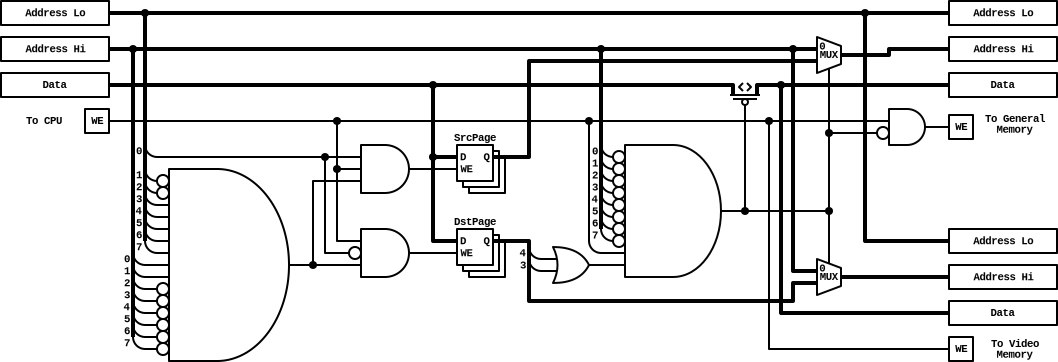
\includegraphics[width=\textwidth]{fvmc}\end{center}

The address bus and write-enable line are forked, with one branch going to the video memory, and the other branch going to all the other memory. The high eight bits of each branch of the address bus are overridden with the contents of the FVMC registers, and the write-enable line is suppressed on the non-video branch. So while the CPU thinks it's writing to zero-page RAM, it's actually triggering a direct memory copy using the data bus, while supplying the low eight bits of the source and destination addresses. Because of a race condition, whether or not the nominally-addressed zero-page memory is changed cannot be garanteed.

The FVMC destination page is set by writing to \texttt{03F8}. Writing a zero to this address disables FVMC. The destination page must be in the range \texttt{08-1F} (video memory) to be effective. The source page is set by writing to \texttt{03F9}, and must not be in the video memory range to be effective.

\section{Interrupts}

Interrupts can be triggered by the video display hardware, as specified by the Video Interrupt Flags, by logic in the cartridge, or by other means not yet determined.\footnote{As of emulator version \oldstylenums{0.1992}d, interrupts are not triggered in any circumstance.} In response to an interrupt event, program execution proceeds from address \texttt{2010}.

\chapter{Programming in High-Level Languages}
\section{Cross-Compiling}

Compilers exist on modern computer systems that generate assembly code for 6502 microprocessors. These ought to be suitable, perhaps with some custom libraries and/or headers, for targeting the Retro 6k Fantasy Computer Entertainment System.

\section{Interpreter Cartridges}

No programming language interpreter cartridges exist at this time. For now, let's consider this a challenge for the reader.

\chapter{Packaging Cartridges for Emulation}
\section{Cartridge Container File Format}

A file describing a Retro 6k cartridge should have a name ending with \texttt{.R6kCart}. The first eight bytes is a magic number, the literal byte sequence \texttt{47 A9 02 6A BB 47 F3 A7}. Following that is the offset (counting from the beginning of the file) to the Page Flags array as a 4-byte little-endian number, then the offset to the beginning of the ROM (or NVM) data contained within the cartridge.

Beginning at offset \texttt{0010} is a sequence of extension data. The extension format has not been determined at this time, except that the byte sequence \texttt{00 00 00 00}, where an extension is expected to begin, indicates that there are no (more) extensions. Extensions will allow for the emulation of cartridges that have more than just memory chips connected directly to the system address \& data buses. Such additional features may include bank switching, a clock that tracks time when the cartridge is unpowered, a label image, and more..

The Page Flags array is 160 bytes which describe what kind of memory, if any, serves each of the 160 pages (\texttt{20-BF}) of cartridge address space. The lowest two bits, taken together, have the following meaning: 0, no memory at this address; 1, read-only memory; 2, random-access memory; 3, non-volatile memory. Bit 2, if set, indicates that this page of memory is subject to bank switching. The upper five bits are not used at this time.

Cartridge ROM and NVM data is stored in the file contiguously. Pages that are not marked as ROM or NVM in the Page Flags array are skipped. The contents of NVM pages, as presented in a cartridge file, represent the state of the cartridge before its first use; the Retro 6k emulator will not modify a cartridge file. Instead, data stored in emulated non-volatile cartridge memory is written to a separate file. Multiple such NVM files may be associated with a single cartridge file, representing multiple physical cartridges containing copies of the same software.

\cleartoverso
\pagestyle{empty}
\vspace*{\stretch{1}}

\noindent\thetitle\hfill\textcopyright2019--20 \theauthor

\end{document}
